\documentclass[12pt,a4paper,twoside,notitlepage]{report}

% Allow large number of packages to be used. Workaround LaTeX limitation.
\usepackage{etex}
\reserveinserts{28}

% Explictly specify character encoding
\usepackage[utf8]{inputenc}

% Change font to Palatino
\usepackage[sc]{mathpazo}
\linespread{1.05}         % apparently Palatino needs more leading space between lines
\usepackage[T1]{fontenc}

% Page formatting
\usepackage[parfill]{parskip} 
\usepackage[margin=1in]{geometry}

% Internationalization: customize to UK English style
\usepackage{csquotes}
\usepackage[UKenglish]{babel}

% Make list environments more configurable
\usepackage{enumitem}

% PROOFREAD ONLY
\usepackage{showidx}
\usepackage[textsize=footnotesize,textwidth=0.8in]{todonotes}
\setlength{\marginparwidth}{0.9in}
\usepackage{todonotes}

\usepackage{gitinfo}

% Hyperlinks
% Note must load url before hyperref
\usepackage[hyphens]{url}

% Citations
\usepackage{varioref}
\usepackage{nameref}
% TODO: What citation style should I use?
\usepackage[backend=biber,bibencoding=UTF-8,style=numeric]{biblatex}
\bibliography{diss.bib}
\DeclareBibliographyCategory{cited}
\AtEveryCitekey{\addtocategory{cited}{\thefield{entrykey}}}
\usepackage{footnote}

%%% Mathematics
\usepackage{amsmath}
\usepackage{amsthm}
\usepackage{amsfonts}
\usepackage{braket}
\usepackage{thmtools}
\usepackage{thm-restate}

%% Theorems
\theoremstyle{plain}
% Define theorem to be numbered by section
% Make lemma and corollary share same counter
\newtheorem{thm}{Theorem}[section]
\newtheorem{lemma}[thm]{Lemma}
\newtheorem{cor}[thm]{Corollary}
% Define style for definitions, remarks
\theoremstyle{definition}
\newtheorem{defn}{Definition}[section]
\newtheorem{assumption}{Assumption}[section]
\theoremstyle{remark}
\newtheorem{remark}{Remark}[section]

\renewcommand{\listtheoremname}{List of theorems and definitions}

%% Some new operators
\DeclareMathOperator*{\argmin}{arg\,min}
\DeclareMathOperator*{\argmax}{arg\,max}

% Figures
\usepackage{verbatim} % environment where formatting preserved exactly
\usepackage{tikz} % language for figures
\usepackage{tikzscale}
\usepackage{pgfplots}

\usepackage{booktabs}
\usepackage{subcaption} 
\usepackage{xcolor}
\usepackage[export]{adjustbox}
\usepackage{graphicx}
\usepackage[justification=centering,font=it]{caption}
\usepackage{colortbl}
\usepackage{tabularx}

\usepackage{changepage}
% wide page for side by side figures, tables, etc
\newlength{\offsetpage}
\setlength{\offsetpage}{2.0cm}
%\newenvironment{widepage}{\begin{adjustwidth}{-\offsetpage}{-\offsetpage}%
%        \addtolength{\textwidth}{2\offsetpage}}%
%    {\end{adjustwidth}}
\newenvironment{widepage}{}{}

\graphicspath{ {./figures/} }
\DeclareGraphicsExtensions{.pdf,.png}
%\newcommand{\includepgf}[1]{\input{./figures/#1.pgf}}

% Formatting of units
\usepackage{siunitx}

% tick and cross marks
% per http://tex.stackexchange.com/questions/42619/x-mark-to-match-checkmark
\usepackage{pifont}
\newcommand{\cmarkcolor}{\color{green}}
\newcommand{\xmarkcolor}{\color{red}}
\newcommand{\mmarkcolor}{\color{blue}}
\newcommand{\cmark}{{\cmarkcolor \ding{51}}}
\newcommand{\xmark}{{\xmarkcolor \ding{55}}}
\newcommand{\mmark}{{\mmarkcolor \tikz \node[draw,circle]{};}}

%\newcommand{\tikzcircle}[2][black,fill=black]{\tikz[baseline=-0.5ex]\draw[#1,radius=#2] (0,0) circle ;}%
%% N.B. Need to add extra {} to make this work, weird
%\newcommand{\circlebad}{\tikzcircle[red,fill=red]{2pt}}
%\newcommand{\circleok}{\tikzcircle[orange,fill=orange]{2pt}}
%\newcommand{\circlegood}{\tikzcircle[green,fill=green]{2pt}}

% colors for percentile figures
\definecolor{matplotlib_blue}{HTML}{00008B}
\definecolor{matplotlib_green}{HTML}{004225}
\definecolor{matplotlib_red}{HTML}{AE0C00}
\definecolor{matplotlib_cyan}{HTML}{00FFFF}

\definecolor{matplotlib_bar_r}{rgb}{1.0,0.6,0.6}
\definecolor{matplotlib_bar_g}{rgb}{0.6,0.8,0.6}
\definecolor{matplotlib_bar_b}{rgb}{0.6,0.6,1.0}
\definecolor{matplotlib_bar_k}{rgb}{0.6,0.6,0.6}

%%% Indexing
%% Hyperref
\usepackage[bookmarks,pdftex,pdfpagelabels,verbose]{hyperref}
% Colour of links, and bio information
\hypersetup{
    colorlinks,
    linkcolor={red!50!black},
    citecolor={blue!50!black},
    urlcolor={blue!80!black},
    pdfauthor = {Adam Gleave},
    pdftitle = {Hapi: fast and scalable cluster scheduling using flow networks},
    pdfcreator = {LaTeX, git commit \gitAbbrevHash}
}

%% Index
\usepackage{makeidx}
\makeindex

%%% Pseudocode and code listings
%% Pseudocode
\usepackage[section]{algorithm} % floating environment
\usepackage[noend]{algpseudocode} % algorithmicx package
% custom commands for algorithmicx
\newcommand*\Let[2]{\State #1 $\gets$ #2}
\newcommand{\Break}{\State \textbf{break} }
\renewcommand{\algorithmicrequire}{\textbf{Precondition:}}
\renewcommand{\algorithmicensure}{\textbf{Postcondition:}}

%% Code listings
\usepackage{listings}
% default listings package configuration for highlighting C code
\lstset{
    language = C,
    basicstyle=\ttfamily,
    keywordstyle=\color[rgb]{0,0,1}\ttfamily\bfseries,
    identifierstyle=\ttfamily,
    stringstyle=\color[rgb]{0.627,0.126,0.941}\ttfamily,
    commentstyle=\color[rgb]{0.133,0.545,0.133}\ttfamily,
    morecomment=[l][\color{magenta}]{\#},
    captionpos=b,
}

\newcommand{\code}[1]{\texttt{#1}}


%%% Cleverref: must load after hyperref, so orphaned
\usepackage{cleveref}
% use \S and \S\S for section references
% SOMEDAY: do we even want the \S symbol?
\makeatletter
\newcommand{\crefformats}[2]{%
    \@for\next:=#1\do{%
        \expandafter\crefformat\expandafter{\next}{#2}%
    }%
}
\makeatother
\makeatletter
\newcommand{\crefnames}[3]{%
    \@for\next:=#1\do{%
        \expandafter\crefname\expandafter{\next}{#2}{#3}%
    }%
}
\makeatother
\newcommand{\crefsections}[0]{
    % override singular case, getting rid of any space
    \crefformats{chapter,section,subsection}{\S##2##1##3}
    \crefformats{appendix,subappendix,subsubappendix}{appendix~##2##1##3}
    % this overrides the default singular case, which has already been overridden; no-op. But replaces plural case with \S\S.
    \crefnames{chapter,section,subsection}{\S}{\S\S}
    \crefnames{appendix,subappendis,subsubappendix}{appendix}{appendices}
}
\crefsections
% Tell cleveref what plural forms for theorems are
\crefname{thm}{theorem}{theorems}
\crefname{lemma}{lemma}{lemmas}
\crefname{cor}{corollary}{corollaries}
\crefname{defn}{definition}{definitions}
\crefname{assumption}{assumption}{assumptions}
\crefname{remark}{remark}{remarks}

% makes line numbers in different algorithms distinguishable from each other
\makeatletter
\newcounter{algorithmicH}% New algorithmic-like hyperref counter
\let\oldalgorithmic\algorithmic
\renewcommand{\algorithmic}{%
    \stepcounter{algorithmicH}% Step counter
    \oldalgorithmic}% Do what was always done with algorithmic environment
\renewcommand{\theHALG@line}{ALG@line.\thealgorithmicH.\arabic{ALG@line}}
\makeatother

% Customize Table of Contents. Don't include list of figures or table of contents in the table of contents. Do still show the bibliography.
\usepackage[nottoc,notlof,notlot]{tocbibind}
% This gives more control over lists of {figures,tables,...} sections
% In particular, it by default disables the (unwanted) page break between them
\usepackage{tocloft}

% Miscellaneous formatting
\raggedbottom					% try to avoid widows and orphans
\sloppy
\clubpenalty 1000
\widowpenalty 1000
\hyphenpenalty 10000
\makeatletter
\pgfdeclareshape{document}{
	\inheritsavedanchors[from=rectangle] % this is nearly a rectangle
	\inheritanchorborder[from=rectangle]
	\inheritanchor[from=rectangle]{center}
	\inheritanchor[from=rectangle]{north}
	\inheritanchor[from=rectangle]{south}
	\inheritanchor[from=rectangle]{west}
	\inheritanchor[from=rectangle]{east}
	\inheritanchor[from=rectangle]{north east}
	\inheritanchor[from=rectangle]{north west}
	% ... and possibly more
	\backgroundpath{% this is new
	% store lower right in xa/ya and upper right in xb/yb
	\southwest \pgf@xa=\pgf@x \pgf@ya=\pgf@y
	\northeast \pgf@xb=\pgf@x \pgf@yb=\pgf@y
	% compute corner of ‘‘flipped page’’
	\pgf@xc=\pgf@xb \advance\pgf@xc by-10pt % this should be a parameter
	\pgf@yc=\pgf@yb \advance\pgf@yc by-10pt
	% construct main path
	\pgfpathmoveto{\pgfpoint{\pgf@xa}{\pgf@ya}}
	\pgfpathlineto{\pgfpoint{\pgf@xa}{\pgf@yb}}
	\pgfpathlineto{\pgfpoint{\pgf@xc}{\pgf@yb}}
	\pgfpathlineto{\pgfpoint{\pgf@xb}{\pgf@yc}}
	\pgfpathlineto{\pgfpoint{\pgf@xb}{\pgf@ya}}
	\pgfpathclose
	% add little corner
	\pgfpathmoveto{\pgfpoint{\pgf@xc}{\pgf@yb}}
	\pgfpathlineto{\pgfpoint{\pgf@xc}{\pgf@yc}}
	\pgfpathlineto{\pgfpoint{\pgf@xb}{\pgf@yc}}
	\pgfpathlineto{\pgfpoint{\pgf@xc}{\pgf@yc}}
	}
}
\makeatother

% footnote without number marker
\newcommand\blfootnote[1]{%
    \begingroup
    \renewcommand\thefootnote{}\footnote{#1}%
    \addtocounter{footnote}{-1}%
    \endgroup
}

\usepackage{layout}

\begin{document}

%\layout

\nocite{*}                      % detect unused references
%\bibliographystyle{acm}		% used ieeetr in the proposal
								% what is the style guide consensus?

%TC:ignore
%%
\pagenumbering{Alph}
\pagestyle{empty}

\hfill{\large \bf Adam Gleave}

\vspace*{30mm}

% Title? Positive words: accurate/optimal/precise; high-performance/fast; 
% High-performance cluster scheduling using flow networks
% Come up with couple of alternatives
% Cluster scheduling at scale: ...
% Data-center scheduling?

\begin{center}
   	%{\Huge \textbf{Hapi}} \\
    {\fontsize{36pt}{1em}\selectfont \textbf{Hapi}} \\
    \large
    \vspace*{2mm}
    \textbf{Fast and scalable cluster scheduling \\ using flow networks} \\
   	\vspace*{10mm}
    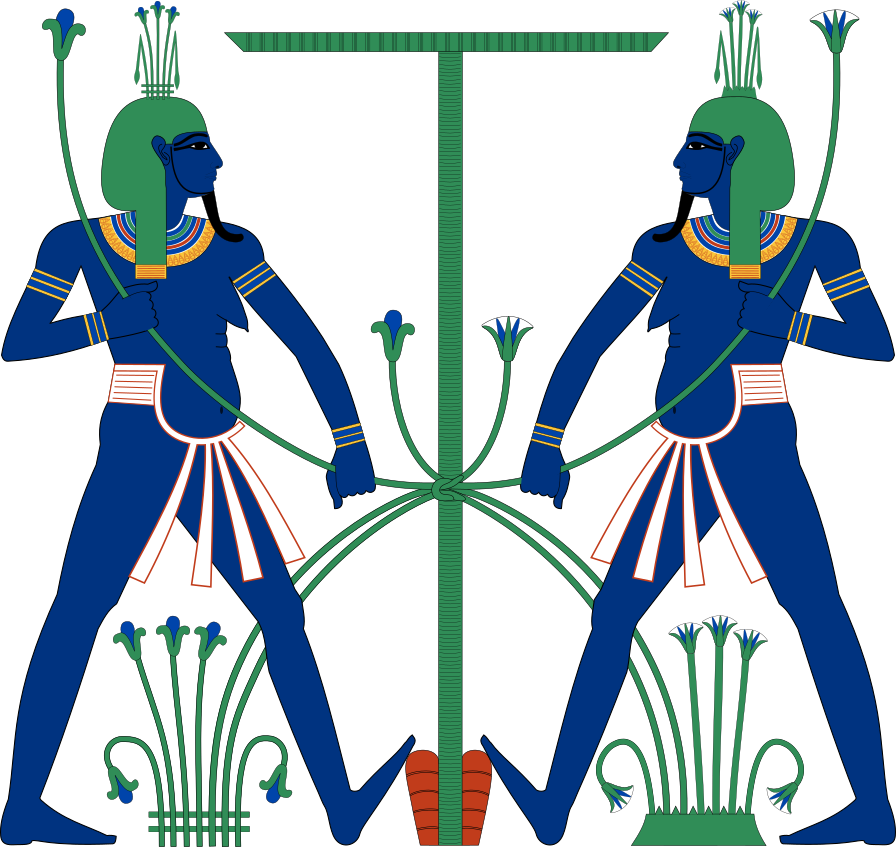
\includegraphics[width=0.35\textwidth]{logo/Hapy_tying} \\
	\vspace*{10mm}
	Computer Science Tripos, Part II \\
	\vspace*{5mm}
	St John's College \\
	\vspace*{5mm}
    % PROOFREAD: DATE
    13\textsuperscript{th} May 2015
\end{center}
\clearpage
\vspace*{\fill}

Hapi is the ancient Egyptian god of the annual flooding of the Nile. The floods were critical to Egyptian agriculture, depositing fertile soil on the river banks. In line with his importance, Hapi was also the god of both upper and lower Egypt. My project's logo depicts this duality, with the double deity tieing together the symbol of upper Egypt (the lotus, on the left) and lower Egypt (the papyrus, on the right).

Much as the Nile was the lifeblood of Egyptian society, cluster schedulers are critical in modern cloud computing applications. After Hapi has solved the flow problem, the scheduler can deliver work to idle machines, in a periodic pattern reminiscent of the Nile's annual floods. I am proud to say Hapi also embodies the duality of its namesake, bringing together the theoretical and applied in computer science similarly to how the deity brought together the two halves of Egypt.

%I am proud to say Hapi also embodies the duality of its namesake, making theoretical advancements to solve a pressing problem in distributed systems research

%Much as the Nile was the lifeblood of Egyptian society, cluster schedulers are critical in modern cloud computing applications. In a pattern reminiscent of the Nile's annual flood, in each periodic scheduling round Hapi sends flow through the network, delivering work to idle machines. This project has a theoretical focus, with most work performed on algorithms for optimisation problems. However, it is motivated by pressing problems in distributed systems research. This duality mirrors that of Hapi, and I am pleased to bring together strands of Computer Science much as Hapi united Egypt.

\blfootnote{The logo is by Jeff Dahl, and is inspired by ancient Egyptian depictions. It is available under the GNU Free Documentation License at \url{http://commons.wikimedia.org/wiki/File:Hapy_tying.svg}.}

\vspace*{\fill}

%%%%%%%%%%%%%%%%%%%%%%%%%%%%%%
% Proforma

\setcounter{page}{1}
\pagenumbering{roman}
\pagestyle{plain}
\chapter*{Proforma}
\vspace*{-2em}
{
	\begin{tabular}{ll}
		Name:			        & \textbf{Adam Gleave}					\\
		College:		        & \textbf{St John's College}\\
        Project Title:	        & \textbf{Hapi: fast and scalable cluster scheduling using flow networks}\\
		Examination:	        & \textbf{Computer Science Tripos, Part II (June 2015)}\\
        Word Count:		        & \textbf{\input{diss-auto-wordcount} \unskip}\\
		Project Originators:	& \textbf{Ionel Gog}\\
        Supervisors:	        & \textbf{Ionel Gog \& Malte Schwarzkopf}\\
	\end{tabular}
}

% move this here so the table above doesn't get extra space added (which I don't want)
\renewcommand{\arraystretch}{1.3}
\vspace*{-1em}
\section*{Original aims of the project}

Recent research into cluster scheduling --- assigning tasks to machines --- has suggested that scheduling can fruitfully be expressed in terms of an optimisation problem over flow networks. The \emph{Hapi} project seeks to develop high-performance algorithms to solve these problems, enabling so-called flow scheduling systems to scale to the largest clusters built today. Implementation and performance analysis of an approximation algorithm forms the core success criteria for \emph{Hapi}. Extensions include development of an incremental solver, which would reuse previous optimal solutions to exploit similarities between successive flow networks.

\vspace*{-1em}
\section*{Work completed}

\emph{Hapi} was highly successful, achieving a $14.5\times$ speedup over state of the art implementations and sub-second scheduling latency on a 12,000 machine cluster. I surpassed the success criteria by developing both an approximate and incremental solver. As far as I am aware, both implementations are the first of their kind. The performance of these solvers was thoroughly evaluated under the Firmament flow scheduling system, including simulation of a cluster based on pubicly available trace data. In addition, approximation yielded a speedup of between $2\text{--}11\times$ on networks arising in other applications, suggesting its use beyond flow scheduling.

\vspace*{-1em}
\section*{Special difficulties}

None.

\newpage

\section*{Declaration}

I, Adam Gleave of St John's College, being a candidate for Part II of the 
Computer Science Tripos, hereby declare that this dissertation and the work 
described in it are my own work, unaided except as may be specified below, and
that the dissertation does not contain material that has already been used to
any substantial extent for a comparable purpose.

\bigskip
\leftline{Signed}
\medskip
% PROOFREAD: DATE
\leftline{Date: 13\textsuperscript{th} May 2015}

\clearpage

\tableofcontents

\listofalgorithms
\listoftables
\listoffigures
%\listoftheorems[ignoreall,show={theorem,lemma,cor,defn,assumption}]

\newpage
\section*{Acknowledgements}

I would like to thank my supervisors, Ionel Gog and Malte Schwarzkopf, for their invaluable advice and encouragement throughout the project.

%%%%%%%%%%%%%%%%%%%%%%%%%%%%%%%%%%%%%%%%%%%%%%%%%%%%%%%%%%%%%%%%
% Chapters
\clearpage	% before we change the page numbering

%TC:endignore
\setcounter{page}{1}
\pagenumbering{arabic}
\pagestyle{headings}

\chapter{Introduction} \label{chap:intro}

\section{Motivation} \label{sec:intro-motivation}
Clusters of commodity machines have become the dominant approach for high-throughput computing. With the adoption of cloud computing, increasing number of applications must be designed to run across clusters rather than individual machines. Making efficient use of these \emph{warehouse-scale computers} is a major challenge in distributed systems research, with considerable practical implications~\cite{WarehouseScale:2009}.

The scheduler coordinates the cluster, choosing the tasks to run on each machine. This can have considerable ramifications on cluster performance and efficiency. For example, throughput is significantly improved by taking into account \emph{data locality}: scheduling tasks on machines close to where their input data is stored. 

Despite their importance, widely-used schedulers leave much to be desired. I would identify two major drawbacks. The first is failing to adapt to different hardware. Some clusters have considerably higher bandwidth interconnects than others. Data locality will be more important in the latter case than the former. The second issue is a lack of policy flexibility. Every application has a unique set of requirements: it should be possible to specify a weighted set of goals to optimize for.

Hadoop, by far the most widely used distributed systems framework, is an excellent example. The Hadoop Fair Scheduler (HFS), as the name suggests, has excellent fairness properties: different users will receive equal shares of the cluster's resources. However, it makes no attempt to achieve data locality. Research systems exist that can provide both~\cite{Zaharia:2010}. However, we would struggle to find a system which could support a third objective, highlighting policy inflexibility. And apart from rudimentary knowledge as to the total number of computational nodes, the HFS runs entirely blind to the underlying hardware.

The Quincy system, developed at Microsoft Research, was designed to address these problems~\cite{Isard:2009}. Quincy builds an explicit model of the data centre, incorporating knowledge about the underlying computational and network hardware. The data centre and the tasks to be scheduled are then represented as a flow network. Solutions to the flow problem correspond to schedules for the tasks.

By modelling the data centre explicitly, Quincy naturally takes into account the idiosyncrasies of different data centres, addressing the first problem. Quincy is also exceedingly flexible, as it does not assume any particular policy. Instead, a cost model must be specified, a procedure to assign a cost to each arc in the network. This allows the policy to be tweaked to achieve a variety of different objectives.

Whilst this so-called "flow scheduling" approach has proven extremely versatile, it has one key weakness. Solving the minimum-cost flow problem to produce an optimal schedule is computationally extremely expensive. This makes the scheduling latency prohibitive for many applications. Even where the latency is tolerable currently, there are concerns about the scalability of the technique. Clusters look set to continue to grow in size. By contrast, the scalar performance of processors is believed to have mostly peaked, and flow algorithms are difficult to parallelise.

In this dissertation, I explore techniques to improve the performance of flow solving algorithms on networks produced by Quincy-style systems. Significant speed-up will enable flow scheduling systems to be adopted in practice, with the consequent performance and efficiency gains in computer clusters.

\section{Challenges} \label{sec:intro-challenges}
Research into the minimum-cost flow problem has been active since the 1950s, owing to its numerous practical applications. There is therefore a considerable body of existing work on the problem, described further in \vref{sec:intro-related-work}. It will be necessary for me to assimilate this large body of existing material before I can attempt to improve upon it.

Given that many seasoned researchers have spent their careers working on this problem, it will be difficult to achieve significant performance improvements. Not only has there been considerable work in developing efficient algorithms, the reference implementations for these algorithms have been extensively hand-optimised.

Whilst the task ahead is daunting, success will enable a new generation of schedulers, able to address the challenges which face today's major technology companies.

\section{Related work} \label{sec:intro-related-work}
Brief literature survey.

\cleardoublepage
\chapter{Preparation} \label{chap:prep}

% Proofread: None/Once

\section{Cluster scheduling} \label{sec:prep-scheduling}

Much as an operating system scheduler maps threads to processor cores, a cluster scheduler maps tasks to computational nodes. I will start by giving a brief overview of the requirements cluster schedulers must meet. Following this, I will summarise the prevailing approaches to scheduling. Finally, I will discuss the principles underlying the Quincy system, and how it improves upon competing schedulers.

\subsection{Design goals} \label{sec:prep-scheduling-goals}

The cluster scheduler is critical to performance. However, it faces a challenging task. There may be tens or hundreds of thousands of machines to manage, with perhaps many more tasks. Furthermore, there are a mind-boggling number of parameters which can impact the efficiency of a schedule. To name just a few, the fine-grained resource requirements (in terms of CPU, memory and IO), the location of its data and the characteristics of the underlying network all play a role. With the shift away from batch to more interactive applications on clusters, scheduling latency is increasingly also a concern~\cite{Ousterhout:2013}. The ideal scheduler therefore needs to place thousands of tasks, taking into account information from a variety of sources, within a sub-second time frame.

How can we judge whether a scheduler is effective? First we must define what we mean by performance. In batch applications, we care primarily about throughput. For interactive applications, low latency is essential. As is often the case, these two objectives are in conflict: a scheduler cannot optimise for both. Most applications will fall somewhere between these two extremes, and will perform best under a scheduler which achieves a compromise between the two objectives.

Once we know our objectives, it remains to consider what data is necessary to find an optimal solution. Clearly, we must take into account the task and its resource requirements. Equally important, but often neglected, is accounting for the resources present in the cluster. Different clusters may call for drastically different scheduling policies. For example, throughput can be significantly improved in many clusters by the scheduler taking into account \emph{data locality}: placing tasks on machines close to where their input data is stored. However, performance is only improved when IO is a bottleneck. In a cluster with a high-bandwidth specialised interconnect such as InfiniBand, performance might actually be harmed by scheduling with data locality in mind, as it may make less efficient use of other resources in the cluster which may be more scarce.

To summarize, for optimal performance the scheduler must be able to adapt itself to different hardware platforms and application requirements. Furthermore, ideally the scheduling latency would be kept low, in order to support interactive applications.

\subsection{Prevailing approaches} \label{sec:prep-scheduling-approaches}

Apache Hadoop is by far the most widely used open-source distributed systems framework. It was originally developed by Yahoo, where it continues to see active use, with their largest cluster having 36,000 cores. Hadoop is also used at Amazon, Facebook and LinkedIn~\cite{HadoopPoweredBy}. Representing the state of the art used in industry, it is instructive to consider the scheduling techniques it utilises. 

Until 2008, Hadoop supported only one scheduler~\cite{HadoopFairSchedulerJIRA}: a simple FIFO queue, executing whichever job had waited longest. This offers high throughput, and so is attractive for batch jobs, Hadoop's traditional application. However, it fares poorly in other applications. In particular, the latency can be very high, as a job (no matter how small) must wait in line between all previously submitted tasks. In addition, their is no notion of fairness: one heavy user of the cluster can starve other users of resources.

Hadoop has chosen to resolve these shortcomings by introducing a pluggable scheduler framework~\cite{HadoopSchedulingIBM}. This is a reflection of the wide variety of application requirements: new schedulers can be written to meet particular needs. The distribution includes two scheduling algorithms, in addition to the original FIFO queue: the Fair Scheduler and Capacity Scheduler. 

The Fair Scheduler was designed at Facebook. It ensures that, over time, each job gets an equal share of available resources. Moreover, it pioneered a technique known as delay-scheduling, allowing the cluster administrator to sacrifice some fairness in order to achieve greater data locality~\cite{Zaharia:2010}. 

The Capacity Scheduler was designed at Yahoo, with the goal of supporting distinct application classes on the same cluster. Hard resource guarantees can be provided to each application class to ensure a minimum service level. At the same time, applications are allowed to burst beyond this level when there are cluster resources idle.

Note both schedulers are designed with specific purposes in mind. Whilst offering good performance in the narrow domains they were designed for, there is little policy flexibility, limiting their applicability more generally. 

Another drawback is that the schedulers run mostly blind to the underlying hardware. The Fair Scheduler is slightly better in this regard, as it takes into account data locality. But this is not enough. Cluster environments are increasingly heterogeneous~\cite{Reiss:2012}, posing problems for traditional schedulers. The LATE scheduler, designed to be robust to heterogenity, improved response times by a factor of 2 over Hadoop's default scheduler when running on Amazon's Elastic Compute Cloud (EC2)~\cite{Zaharia:2008}. Even in more homogeneous environments, network topology and capacity can be highly important, as discussed in~\S\ref{sec:prep-scheduling-goals}.

Hitherto, I have considered the state of the art amongst schedulers that are in the public domain. Clusters are indispensable assets to today's major web companies, and consequently there is considerable research into this area in industry as well as academia. Owing to the competitive nature of the industry, unfortunately the details of the schedulers used by major technology firms such as Google are trade secrets. Naturally, this makes it difficult to evaluate the state of the art within industry. 

However, the information which is public suggests that the same basic approaches we have seen above are in use in industry. The designs may, of course, have been tweaked to meet specific application requirements, and to work efficiently on the cluster architectures favoured by the respective technology firm. For example, the Google scheduler allows tasks to specify a kernel version constraint, and attempts to minimise peak power demand by load balancing. Apart from idiosyncrasies such as these, the approach is broadly similar to published research systems~\cite[\S2.1]{Sharma:2011}.

\subsection{Quincy and related systems} \label{sec:prep-scheduling-quincy}

Despite considerable research effort, both in industry and academia, the traditional scheduler designs discussed above suffer from two major deficiencies. The first is a lack of policy flexibility. Hadoop attempts to solve this by allowing for an ecosystem of different schedulers, but this approach is limited. As we try to trade-off more objectives, there is a combinatorial explosion in the number of scheduler designs needed. The second problem is a failure to take the underlying cluster architecture into account when making scheduling decisions.

% Nice example from Malte's PhD thesis of three-way relationship between data locality, fair resource sharing and scheduling delay. Could use this or something similar to illustrate this?

Microsoft Research developed the Quincy system~\cite{Isard:2009} to address these problems. Working with the Dryad distributed execution engine~\cite{Isard:2007}\footnotemark, the Quincy scheduler builds a model of the cluster and the tasks. A flow network is generated from this model, with solving the flow problem dual to finding a schedule.
\footnotetext{Dryad allows tasks ("computational vertices") to be connected together by communication "channels" to form an (acyclic) dataflow graph. Other computational frameworks, such as MapReduce and relational algebra, reduce to special cases of Dryad.}

In the configuration described in the original paper, Quincy optimised for high levels of data locality and fairness. Its performance in this regard was admirable. Quincy's throughput was 40\% greater than that of standard queue-based approaches, such as those used by Hadoop. Moreover, data transfer was reduced by up to a factor of 3.9. This could allow for considerable cost savings when building out clusters, by reducing the interconnect capacity required.

% TODO: Any other papers that are relevant in this regard?
Since the paper introducing Quincy was published in 2009, new scheduling algorithms designed specifically with data locality and fairness in mind have been published~\cite{Guo:2012,Jin:2011,Ibrahim:2010}. Although no up-to-date empirical evaluation is available, my suspicion is Quincy would no longer lead the pack in this regard. The power of Quincy is not, however, in being yet another scheduler optimised for a narrow domain. Rather, it is that the system offers an extremely high level of flexibility.

As we saw above, most schedulers focus on one or two specific goals. There may be some degree of configurability: the Hadoop Fair Scheduler, for instance, allows the administrator to control the trade-off between fairness and data locality. Quincy, by contrast, is almost infinitely configurable. Indeed, the scheduler does not assume any specific policy. Instead, the policy is defined by a cost model: a procedure which assigns costs to arcs in the flow network.

It would be an overstatement to say that all policies can be expressed in this way: flow networks are not Turing complete. Indeed, there is a concrete counterexample of this. In gang scheduling\footnotemark, a constraint is added that pairs of tasks must be scheduled to run simultaneously. This is difficult or impossible to express in this model: flows in a network are inherently independent.
\footnotetext{Note gang scheduling does not benefit systems such as Dryad. It is most useful when there is bidirectional communication between the two tasks. This would correspond to a cycle in the dataflow graph, which is explicitly disallowed.}

However, cases such as these are the exception that proves the rule. In practice, the model is very powerful, allowing a range of scheduling policies to encoded in terms of cost models. Moreover, the policies naturally tend to adapt themselves to different cluster architectures, as the topology of the flow network will also adjust itself.

% TBC: Add reference to Firmament

\section{Flow networks} \label{prep-flow}

Before we discuss how Quincy encodes scheduling in terms of a flow network, we must pause to formalise the notion of a flow network and the associated flow problems, and establish the notation to be used throughout the rest of the dissertation. After this, I will summarise properties of flow networks which will be needed later when analysing and designing flow algorithms.

\subsection{Introduction}

\subsubsection{Definitions and notation}

A \emph{flow network} is a weakly connected\footnotemark directed graph $G=(V,E)$.
\footnotetext{A directed graph is weakly connected if the undirected graph formed by replacing all directed edges with undirected edges is itself connected.}

Each arc $(i,j)\in E$ has an associated \emph{capacity} (or \emph{upper	bound}\footnotemark) $u_{ij}$, and a \emph{cost} $c_{ij}$.
\footnotetext{Some authors also include a lower bound $l_{ij}$. This will not feature in flow scheduling. Moreover, any network featuring lower bounds can be transformed into an equivalent one where all lower bounds are zero. \cite[p.~39]{Ahuja:1993}}

Each node $i\in V$ has an associated supply/demand $b_{i}$. Node $i$ is said to be a \emph{supply node} if $b_{i}>0$, a \emph{demand	node} if $b_{i}<0$ and a \emph{transshipment node} if $b(i)=0$.

The problems we will consider involve finding a solution vector $\mathbf{x}$,
specifying the flow $x_{ij}$ at each arc $(i,j)\in E$. A solution
$\mathbf{x}$ is \emph{feasible}, and we say it is a \emph{flow}, if it satisfies capacity constraints at every arc:

\begin{equation} \label{eq:capacity-constraints}
0\leq x_{ij}\leq u_{ij}\:\forall(i,j)\in E
\end{equation}

and mass balance constraints at each node:

\begin{equation} \label{eq:mass-balance}
\sum_{j\::\:(i,j)\in E}x_{ij}-\sum_{j\::\:(j,i)\in E}x_{ji}=b(i)\:\forall i\in V
\end{equation}

That is, the net flow out of the node is exactly equal to the supply
at that node (which may be negative.)

\subsubsection{Assumptions}

\begin{assumption}[Integrality] \label{assumption:integrality}
All quantities defining the flow network take on only integer values.\end{assumption}
    
Note any network with rational quantities can be transformed into an equivalent integral network, by multiplying throughout by the greatest common denominator. Meanwhile, flow algorithms may not terminate on irrational data, so there is little point considering this case. Fortunately, the networks produced by systems such as Quincy are naturally integral, since quantities such as resource consumption in a data centre are inherently discrete. \\

\begin{assumption}[Non-negative arc costs] \label{assumption:non-negative-arc-costs}
For all $(i,j) \in E$, $c_{ij} \geq 0$.\end{assumption}

~

\begin{remark} 
This assumption is without loss of generality\footnote{Any network with negative arc costs can be transformed into an equivalent one with non-negative arc costs. For each arc $(i,j) \in E$ with a negative cost, replace the flow variable $x_{ij}$ with the variable $u_{ij} - x_{ji}$. Arc $(j,i)$ then replaces arc $(i,j)$, and $c_{ji} = -c_ij \geq 0$. \cite[p.~48]{Ahuja:1993}}.
\end{remark}

\begin{cor}All quantities defining arcs take on only values from the natural numbers.\footnotemark
\footnotetext{To avoid confusion, I will follow the convention $0\in\mathbb{N}$ throughout this document.}
\end{cor}
\begin{proof}
Every arc is defined by its capacity and its cost. Capacities are non-negative by definition, and arc costs are non-negative by \cref{assumption:non-negative-arc-costs}. This together with \cref{assumption:integrality} guarantee capacities and costs are natural numbers.
\end{proof}

We can therefore use exclusively unsigned integer data types when representing arcs in computer code.

\subsubsection{The minimum-cost flow problem} \label{sec:prep-flow-mcf}

The well-known maximum flow problem involves finding a solution vector
$\mathbf{x}$ subject to constraints (1) and (2), i.e. finding a feasible
flow.

Our focus will be on a generalization of this, known as the minimum
cost problem. Formally, it is:

\begin{equation} \label{eq:mcf-primal-problem}
\mbox{minimise}\ s(\mathbf{x})=\sum_{(i,j)\in E}c_{ij}x_{ij}
\end{equation}
where $\mathbf{x}$ is constrained to be a feasible flow. A feasible
flow $\mathbf{x}$ minimizing the above quantity is said to be \emph{optimal}.

In general, there may be no feasible solution to a network. For example,
the problem may be imbalanced: $\sum_{i\in V}b_{i}\neq0$. All networks
produced by the Quincy system are guaranteed to be solvable, however,
so this does not concern us. Consequently, I will assume in subsequent
discussions that networks are feasible, unless stated otherwise%
\footnote{For robustness, however, all algorithms implemented as part of this project detect if a network is infeasible.}.

\subsection{Scheduling using flows}

% Previously have described the advantages of Quincy, and roughly its architecture, but not gone into any technical detail.
% Intro: models scheduling as an optimisation problem, the minimum-cost flow problem.
% Flow from tasks (source nodes) to machines or unscheduled aggregators, draining to a sink
% Capacities specify possible scheduling states of tasks: e.g. enforce minimum number of tasks scheduled per job
% Costs specify preferences

Quincy and Firmament frame scheduling in terms of the minimum-cost flow problem. \emph{Jobs} are submitted to the scheduler, each consisting of a number of \emph{tasks}. Flow drains from task nodes to a sink node. Along the way, it passes either through a machine node (indicating the task is to be placed there) or a special job unscheduled aggregator node (indicating the task is to be left unscheduled).

Arc capacities are used to \emph{restrict} the possible scheduling assignments. The costs associated with arcs, by contrast, specify \emph{preferences} between possible scheduling assignments. Different scheduling policies may be encoded by varying the costs.

\subsubsection{Network structure}
%TBC: Table here would really help
%TBC: Flow graphs really useful here! Illustrate each type of network.

Each task $i$ in job $j$ is represented by a node $\mathbf{T}_i^j$, with a single unit of supply. Machines are represented by nodes $\mathbf{M}_l$, with arcs to a sink node $\mathbf{S}$. Task nodes have arcs to machine nodes, with a cost specifying the preference of being scheduled on that machine.

There is a problem with this scheme: if there are more tasks submitted than can be scheduled, the flow problem would become unfeasible. To fix this, we introduce \emph{unscheduled aggregators} $\mathbf{U}^j$ for each job $j$, with an arc to $\mathbf{S}$. Each task node $\mathbf{T}_i^j$ also has an arc to its unscheduled aggregator $\mathbf{U}_j$, with a cost specifying the penalty for being unscheduled.

In the model above, every task has an arc to every machine. Whilst this allows for the model to be highly precise, it is very inefficient\footnotemark. Quincy makes the modification of introducing \emph{rack aggregator} nodes $\mathbf{R}_k$, each with an arc to every machine in that rack. Moreover, there is a single \emph{cluster aggregator} $\mathbf{X}$ with an arc to every rack aggregator\footnotemark. Each task then has a fixed number of arcs. Some of these may be to individual machines, some to rack aggregators and every task has an arc to the cluster aggregator. 
\footnotetext{The number of arcs will scale linearly with the number of machines. But, of course, as the size of a cluster grows the number of tasks being scheduled will also tend to grow proportionally. So the number of arcs actually will tend to grow \emph{quadratically} with increases in the number of machines. Scalability is a key concern, making this is highly undesirable.}
\footnotetext{Of course, this hierarchical scheme could be extended to any number of levels.}

This scheme of rack aggregators is particularly suited to Quincy. Its cost model is based in large upon the amount of network bandwidth used by a task, which will be similar within a rack. This approach may work less well for other cost models. Firmament generalised this method by introducing \emph{equivalence classes}, both for task and machine\footnotemark nodes, with an aggregator node for entities within an equivalence class.
\footnotetext{In fact, Firmament supports representing resources at a finer grain than machines: for example, an individual core. So machines may themselves be aggregator nodes.}

\subsubsection{Capacities}

Every arc leaving a task node $\mathbf{T}_i^j$ has unit capacity. Note $\mathbf{T}_i^j$ has unit supply and no incoming arcs, so any (non-zero) capacity would be equivalent to unit capacity.

The arcs $\mathbf{M}_l \to \mathbf{S}$ from machine nodes to the sink node have capacity $K$, where $K$ is a parameter specifying the number of tasks which may concurrently run on a machine\footnotemark.
\footnotetext{In the original Quincy system, $K=1$. However, this is clearly a poor utilisation of modern multi-core machines. In fact, performance may often be improved by setting $K > \text{\# of cores}$, on simultaneous multi-threading (SMT) machines.}

The arcs $\mathbf{R}_k \to \mathbf{M}_l$ from rack aggregators to nodes representing their constituent machines also have capacity $K$, since up to $K$ jobs may be scheduled on each machine in the rack via the aggregator. The arcs $\mathbf{X} \to \mathbf{R}_k$ have capacity $mK$, where $m$ is the number of machines in each rack.

The arcs $\mathbf{U}^j \to \mathbf{S}$ can be set to be uncapacitated, allowing any number of tasks in job $j$ to be unscheduled. It is possible, however, to enforce a lower bound $E_j$ and upper bound $F_j$ on the number of tasks that can be scheduled for each job. This is used in Quincy and Firmament. It can provide some degree of fairness, and in particular specifying $E_j \geq 1$ ensures starvation freedom.

Let $N_j$ be the number of tasks submitted for job $j$. To enforce the upper bound $F_j$, give $\mathbf{U}^j$ a demand of $N_j - F_j$. At least this many tasks in job $j$ must then be left unscheduled, guaranteeing no more than $F_j$ tasks are scheduled.

To enforce the lower bound, we set the capacity on $\mathbf{U}^j \to \mathbf{S}$ to $F_j - E_j$. The maximum number of unscheduled tasks is thus the $N_j - F_j$ which are absorbed at $\mathbf{U}^j$, plus the $F_j - E_j$ draining via $\mathbf{U}^j \to \mathbf{S}$. This gives an upper bound of $N_j - E_j$ unscheduled tasks, guaranteeing that at least $E_j$ tasks remain scheduled.

\subsubsection{Cost models}  

% TODO: Firmament supports more cost models, such as Octopus. Will this be in PhD/can I cite it?
A key benefit to the flow scheduling approach is policy flexibility: support for a policy can be added simply by providing a new cost model. The cost model used in the original Quincy system attempts to achieve \emph{data locality}: scheduling tasks close to their input data, in order to minimise network traffic. Firmament includes three other cost models~\cite[ch.~5]{Schwarzkopf:2015}. The Whare-Map and Coordinate Co-Location models aim to improve the utilisation of the cluster by avoiding co-location interference and taking into account the heterogeneity of available resources. The Energy-Aware cost model seeks to achieve energy efficiency whilst meeting application performance guarantees, in a hypothetical heterogeneous cluster containing a mixture of high performance (but low efficiency) and medium performance (but high efficiency) machines.

Given such a variety of possible policies, the solver developed in this project must be independent of any particular cost model. However, having an intuition for how cost models operate is valuable. For reasons of brevity, I will only summarize the cost model in the original Quincy system. Further details of this cost model are available in~\cite{Isard:2009}. A description of the other cost models mentioned above is in~\cite[ch.~5]{Schwarzkopf:2015}.

\paragraph{Quincy cost model}
\begin{table}
    \begin{tabular}{c|c|l}
        \hline 
        Cost & Edge & Meaning\tabularnewline
        \hline 
        \hline 
        $v_{i}^{j}$ & $\mathbf{T}_{i}^{j}\to\mathbf{U}^{j}$ & Cost of leaving task $\mathbf{T}_{i}^{j}$ unscheduled\tabularnewline
        \hline 
        $\alpha_{i}^{j}$ & $\mathbf{T}_{i}^{j}\to\mathbf{X}$ & Cost of scheduling on worst possible machine\tabularnewline
        \hline 
        $\rho_{i,l}^{j}$ & $\mathbf{T}_{i}^{j}\to\mathbf{R}_{l}$ & Cost of scheduling on worst machine in rack $\mathbf{R}_{l}$\tabularnewline
        \hline 
        $\gamma_{i,m}^{j}$ & $\mathbf{T}_{i}^{j}\to\mathbf{M}_{m}$ & Cost of scheduling on machine $\mathbf{M}_{m}$\tabularnewline
        \hline 
    \end{tabular}
    \caption{Costs in the Quincy model}
    \label{table:quincy-costs}
\end{table}

\begin{table}
    \begin{tabular}{c|l}
        \hline 
        Variable & Meaning\tabularnewline
        \hline 
        $\chi^{X}\left(\mathbf{T}_{i}^{j}\right),\chi_{l}^{R}\left(\mathbf{T}_{i}^{j}\right),\chi_{m}^{M}\left(\mathbf{T}_{i}^{j}\right)$ & Data transfer for task $\mathbf{T}_{i}^{j}$ across the core switch.\tabularnewline % if: scheduled on worst possible computer in cluster, scheduled on worst possible computer in rack $\mathbf{R}_{l}$ or scheduled on computer $\mathbf{M}_{m}$ respectively.
        $\mathcal{R}^{X}\left(\mathbf{T}_{i}^{j}\right),\mathcal{R}_{l}^{R}\left(\mathbf{T}_{i}^{j}\right),\mathcal{R}_{m}^{M}\left(\mathbf{T}_{i}^{j}\right)$ & Data transfer for task $\mathbf{T}_{i}^{j}$ across the top-of-rack switch.\tabularnewline
        $\theta_{i}^{j}$ & Number of seconds $\mathbf{T}_{i}^{j}$ has spent scheduled.\tabularnewline
        $\nu_{i}^{j}$ & Number of seconds task $\mathbf{T}_{i}^{j}$ has spent unscheduled.\tabularnewline
        \hline
    \end{tabular}
    \caption{Variables in the Quincy model}
    \label{table:quincy-variables}
\end{table}

\begin{table}
    \begin{tabular}{c|l}
        \hline 
        Parameter & Meaning\tabularnewline
        \hline 
        \hline 
        $\epsilon$ & Cost of transferring 1 GB across core switch\tabularnewline
        \hline 
        $\psi$ & Cost of transferring 1 GB across top of rack switch\tabularnewline
        \hline 
        $\omega$ & Wait-time cost factor for unscheduled aggregators\tabularnewline
        \hline 
    \end{tabular}
    \caption{Parameters for the Quincy model}
    \label{table:quincy-parameters}
\end{table}

The arc costs specified by the model are given in \cref{table:quincy-costs}. All arcs not mentioned in this table have a cost of zero\footnotemark.
\footnotetext{In particular, arcs leaving aggregator nodes, and arcs incoming to the sink, both have zero cost.}

The model assumes the data processed by tasks resides in a distributed file system. Each machine in the cluster can access any object in the file system, by fetching the data from a remote machine. However, retrieving an object from a machine in another rack is more expensive -- both in terms of request latency and network resources consumed -- than transferring the data from a neighbouring machine. Reading the data from a directly connected disk is cheaper still. The Quincy scheduler quantifies these data transfer costs for each scheduling assignment. It then finds an assignment minimising the global data transfer cost across the cluster, in order to achieve data locality.

\Cref{table:quincy-variables} gives the variables maintained by the Quincy scheduler. All arc costs are functions of these variables. The system breaks down the data transfer of a task $\mathbf{T}_{i}^{j}$ into two components: transfer across the core switch, $\chi\left(\mathbf{T}_{i}^{j}\right)$, and top of rack switches, $\mathcal{R}\left(\mathbf{T}_{i}^{j}\right)$. For a particular machine $\mathbf{M}_m$, the data transfer $\chi_{m}^{M}\left(\mathbf{T}_{i}^{j}\right)$ and $\mathcal{R}_{m}^{M}\left(\mathbf{T}_{i}^{j}\right)$ can be computed exactly. However, when it comes to determining the cost of arcs to aggregator nodes $\mathbf{R}_l$ or $\mathbf{X}$, an exact figure is not possible. Instead, we take a conservative upper bound: the \emph{greatest} data transfer that results from scheduling $\mathbf{T}_{i}^{j}$ on the \emph{worst} machine in rack $\mathbf{R}_l$ or the cluster as a whole, respectively.

The system also keeps track of the time $\theta_i^j$ and $\nu_i^j$ a task spends scheduled and unscheduled, respectively. If the task is stopped and then restarted, these times continue to accumulate. This property is needed to guarantee the scheduler makes progress.

Quincy is controlled by three simple parameters, given in \cref{table:quincy-parameters}. $\epsilon$ and $\psi$ specify the cost of data transfers across core and top of rack switches respectively. In general, we would expect $\epsilon > \psi$, since the core switch is more likely to become a bottleneck. $\omega$ controls the penalty for leaving a task unscheduled\footnotemark. Increasing $\epsilon$ and $\psi$ will cause the scheduler to more aggressively optimise for data locality. Increasing $\omega$ will 
\footnotetext{It is possible to vary $\omega$ between jobs in order to encode a notion of priority.}

We are now ready to give formulae for the arc costs given in \cref{table:quincy-costs}. First, let us define the data transfer cost:
\[d_{b}^{A}\left(\mathbf{T}_{i}^{j}\right) = \epsilon\chi_{b}^{A}\left(\mathbf{T}_{i}^{j}\right)+\psi\mathcal{R}_{b}^{A}\left(\mathbf{T}_{i}^{j}\right)\]

The cost of scheduling on the worst machine in the cluster and the worst machine in rack $\mathbf{R}_l$ follow simply:
\[\alpha_{i}^{j} = d^X\left(\mathbf{T}_{i}^{j}\right)\]
\[\rho_{i}^{j,l} = d^R_l\left(\mathbf{T}_{i}^{j}\right)\]
It is tempting to use the same form for the cost, $\gamma^j_{i,m}$ of scheduling on a particular machine $\mathbf{M}_m$. When $\mathbf{T}_{i}^{j}$ is not running on $\mathbf{M}_m$ (either it is unscheduled, or is running on a different machine), this is valid. However, this formula is inappropriate when $\mathbf{T}_{i}^{j}$ is already scheduled on  $\mathbf{M}_m$.

When the task has already been running, $d^M_m\left(\mathbf{T}_{i}^{j}\right)$ will overestimate the cost of the remaining data transfer. To account for the work already invested in $\mathbf{T}_{i}^{j}$, we subtract the time it has been running, giving:
\[\gamma_{i,m}^{j} = d_{m}^{M}\left(\mathbf{T}_{i}^{j}\right)-\begin{cases}
\theta_{i}^{j} & \text{if \ensuremath{\mathbf{T}_{i}^{j}}running on \ensuremath{\mathbf{M}_{m}}}\\
0 & \text{otherwise}
\end{cases}\]

The only remaining cost is $v_i^j$, the penalty associated with leaving a task $\mathbf{T}_{i}^{j}$ unscheduled. We set it proportional to the length of time it has been unscheduled:
\[v_i^j = \omega\nu_{n}^{j}\]

\subsubsection{Properties of these networks}

\begin{lemma} \label{lemma:network-num-nodes}
Let $n$ denote the number of nodes in the network. Then $n = \Theta\left(\text{\# machines} + \text{\# tasks}\right)$.
\end{lemma}
\begin{proof}
There is one node $\mathbf{T}_i^j$ for every task and one node $\mathbf{M}_m$ for every machine, so trivially $n = \Omega\left(\text{\# machines} + \text{\# tasks}\right)$.

It remains to show $n = O\left(\text{\# machines} + \text{\# tasks}\right)$. Consider each class of node in turn.

As stated above $\text{\# task nodes} = \text{\# tasks}$ and $\text{\# machine nodes} = \text{\# machines}$. There is an unscheduled aggregator $\mathbf{U}^j$ for each job $j$. Certainly $\text{\# jobs} = O\left(\text{\# tasks}\right)$. There is at least one machine in every rack, so $\text{\# rack aggregator nodes} = O\left(\text{\# machines}\right)$. 

In addition, there is also a cluster aggregator node $\mathbf{X}$ and sink node $\mathbf{S}$ which are independent of the number of tasks and machines, contributing $O(1)$ nodes.

Thus:
\[n = O\left(\text{\# tasks} + \text{\# machines} + 1\right) = O\left(\text{\# tasks} + \text{\# machines}\right)\]

Hence:
\[n = \Theta\left(\text{\# machines} + \text{\# tasks}\right)\]
\end{proof}

\begin{lemma} \label{lemma:network-num-arcs}
Let $m$ denote the number of arcs in the network. Then $m = O(n)$. That is, the network is \emph{sparse}.
\end{lemma}
\begin{proof}
Consider the outgoing arcs from each class of node. Since every arc is outgoing from exactly one node, this will count every node exactly once.

Each machine $\mathbf{M}_l$ and unscheduled aggregator $\mathbf{U}^j$ has a single outgoing arc, to sink node $\mathbf{S}$. This contributes $O\left(\text{\# machines}\right)$ arcs. The sink node $\mathbf{S}$ has no outgoing arcs.

Rack aggregators $\mathbf{R}_l$ have outgoing arcs to each machine in their rack. Each machine is present in exactly one rack, so these contribute collectively $O\left(\text{\# machines}\right)$ arcs. The cluster aggregator $\mathbf{X}$ has outgoing arcs to each rack; since $O\left(\text{\# racks}\right) = O\left(\text{\# machines}\right)$, this contributes $O\left(\text{\# machines}\right)$ arcs.

It remains to consider task nodes $\mathbf{T}_i^j$. The number of arcs leaving the task node has a constant upper bound. The system computes a \emph{preference list} of machines and racks, and includes arcs only to those nodes (and the cluster aggregator $\mathbf{X}$). Thus this contributes $O\left(\text{\# tasks}\right)$ arcs.

Hence:
\[m = \left(\text{\# machines} + \text{\# tasks}\right)\]
By \cref{lemma:network-num-nodes}, it follows:
\[m = O(n)\]
\end{proof}

\begin{remark}
In fact we have $m = \Theta(n)$: the network is connected so certainly $m = \Omega(n)$. However, we will only use the bound $m = O(n)$.\\
\end{remark}

\begin{lemma} \label{lemma:network-supply}
The largest supply in the network is a unit supply.
\end{lemma}
\begin{proof}
The only nodes in the network with any supply are the task nodes, $\mathbf{T}_i^j$. These by definition have unit supply.
\end{proof}

\begin{remark}
Most nodes in the network are transshipment nodes, with no demand nor supply. The demand nodes in the network are the sink node $\mathbf{S}$ and (optionally) unscheduled aggregators, $\mathbf{U}^j$. These may have a greater than unit demand.
\end{remark}

\subsection{Further definitions and properties}

\subsubsection{Pseudoflows} \label{sec:prep-flow-pseudo}

Whilst all flow algorithms must return a feasible solution, many operate
by manipulating \emph{pseudoflows} in intermediate stages. A pseudoflow
is a vector $\mathbf{x}$ which satisfies the capacity constraints
\cref{eq:capacity-constraints}, but which may not satisfy the mass balance constraints \cref{eq:mass-balance}.

We define the \emph{excess} at a node $i\in V$ to be:

\begin{equation}
e_{i}=b_{i}+\sum_{j\::\:(j,i)\in E}x_{ji}-\sum_{j\::\:(i,j)\in E}x_{ij}
\end{equation}

Node i is said to be an \emph{excess node} if $e_{i}>0$, and a \emph{deficit
	node} if $e_{i}<0$ (with deficit $-e_{i}$). If $e_{i}=0$, $i$
is said to be \emph{balanced}. Note the mass balance constraints hold if and
only if all nodes are balanced.

\subsubsection{Residual networks}

Also important to many flow algorithms is the notion of \emph{residual}
\emph{networks. }The residual network is defined with respect to the
original flow network $G$ and a (pseudo)flow $\mathbf{x}$, and is
denoted by $G_{\mathbf{x}}$. Informally, it represents the actions
an algorithm can take to modify the (pseudo)flow $\mathbf{x}$. In
the case where $\mathbf{x=0},$ we have $G_{\mathbf{0}}=G$.

Formally, we define $G_{\mathbf{x}}=\left(V,E_{\mathbf{x}}\right)$
to be a directed graph where:
\begin{equation}
E_{\mathbf{x}}=\left\{ (i,j)\in V^{2}\::\:(i,j)\in E\land x_{ij}<u_{ij}\right\} \cup\left\{ (j,i)\in V^{2}\::\:(j,i)\in E\land x_{ij}>0\right\} 
\end{equation}


The former set consists of \emph{forward arcs}, which were present
in the original flow network. An arc $(i,j)$ which is saturated,
i.e. $x_{ij}=u_{ij}$, drops out of the residual network. The latter
set consists of \emph{backward arcs}, the reverse of arcs in the original
network. Only arcs with positive flow in the original network have
a corresponding backwards arc.

We define the \emph{residual capacity} of an arc $(i,j)\in E_{\mathbf{x}}$
to be:

\begin{equation}
r_{ij}=\begin{cases}
u_{ij}-x_{ij} & ,\:(i,j)\:\mbox{is a forward arc}\\
x_{ij} & ,\:(i,j)\:\mbox{is a reverse arc}
\end{cases}
\end{equation}

We define the cost of a forward arc $(i,j)$ to be $c_{ij}$, and
a reverse arc $(j,i)$ to be $-c_{ij}$.


\subsubsection{Reduced cost and duality} \label{sec:prep-flow-rc-and-dual}

We may associate with each node $i\in V$ a \emph{potential}, $\pi_{i}$.

\begin{defn}[Reduced costs] \label{defn:reduced-costs}
The \emph{reduced cost} of an arc $(i,j)\in E$ with respect to a
potential $\boldsymbol{\pi}$ is defined as:
\begin{equation}
c_{ij}^{\boldsymbol{\pi}}=c_{ij}-\pi_{i}+\pi_{j}
\end{equation}
\end{defn}

Every linear programming problem, referred to as a \emph{primal} problem,
can be converted to a \emph{dual} problem. Solutions to the dual problem
give an upper bound on the objective value of the primal problem.

The primal version of the minimum-cost flow problem is stated in \S\ref{sec:prep-flow-mcf}. The dual problem is:

\begin{equation}
\mathrm{maximise}\; w(\boldsymbol{\pi})=\sum_{i\in V}b_{i}\pi_{i}-\sum_{(i,j)\in E}\max\left(0,-c_{ij}^{\pi}\right)u_{ij}
\end{equation}

with no constraints on $\boldsymbol{\pi}$.

It can be computationally more efficient to solve the dual problem
rather than the primal problem. Many flow algorithms adopt a dual
approach, or a hybrid of a primal and dual approach.

\subsubsection{Optimality conditions} \label{prep:flow-optimality}

Below, I give conditions on a solution vector $\mathbf{x}$ which
imply it is optimal. These conditions suggest algorithms for solving
the problem. Moreover, they can be used in testing, to verify that
a solution is indeed optimal.\\

\begin{thm}[Negative cycle optimality conditions] \label{thm:optimality-neg-cycle}
A flow $\mathbf{x}$ is an optimal solution to the minimum-cost flow problem if and only if the residual network $G_\mathbf{x}$ has no negative cost (directed) cycle.
\end{thm}
\begin{proof}
See~\cite[p.~307]{Ahuja:1993}.
\end{proof}

\begin{thm}[Reduced cost optimality conditions] \label{thm:optimality-reduced-cost}
Let $\mathbf{x}$ be a feasible solution. It is an optimal solution
to the minimum-cost flow problem if and only if there exists a node
potential vector $\boldsymbol{\pi}$ such that that the reduced cost
of each arc in the residual network $G_{\mathbf{x}}$ is non-negative:

\begin{equation} \label{eq:optimality-reduced-cost}
c_{ij}^{\boldsymbol{\pi}}\geq0\:\forall(i,j)\in E_{\mathbf{x}}
\end{equation}
\end{thm}
\begin{proof}
See~\cite[p.~309]{Ahuja:1993}.
\end{proof}

\begin{thm}[Complementary slackness optimality conditions] \label{thm:optimality-complementary-slackness}
Let $\mathbf{x}$ be a feasible solution. It is an optimal solution
to the minimum-cost flow problem if and only if there exists a node
potential vector $\boldsymbol{\pi}$ such that for every arc $(i,j)\in E$:

\begin{equation}
\text{if \ensuremath{c_{ij}^{\boldsymbol{\pi}}>0}, then \ensuremath{x_{ij}=0}}
\end{equation}

\begin{equation}
\text{if \ensuremath{c_{ij}^{\boldsymbol{\pi}}<0}, then \ensuremath{x_{ij}=u_{ij}}}
\end{equation}

\begin{equation}
\text{if \ensuremath{c_{ij}^{\boldsymbol{\pi}}=0}, then \ensuremath{0\leq x_{ij}\leq u_{ij}}}
\end{equation}
\end{thm}
\begin{proof}
This can easily be seen to be equivalent to the reduced cost optimality conditions, by expanding out \cref{eq:optimality-reduced-cost} using the definition of a residual network and performing a case analysis. A detailed proof is given in~\cite[p.~310]{Ahuja:1993}. 
\end{proof}

\subsubsection{Notation for complexity analysis} \label{sec:prep-flow-complexity}

Some notation will be useful when it comes to analysing the asymptotic complexity
of algorithms. 

Let $n=|V|$ and $m=|E|$ denote the number of nodes and arcs respectively.

The running time of algorithms depends not just on the size of the
network, but also on the magnitudes of input data. Let $U$ denote
the largest node supply/demand, or arc capacity:
\begin{equation}
U=\max\left(\max\left\{ |b_{i}|\::\: i\in V\right\} ,\max\left\{ u_{ij}\::\:\left(i,j\right)\in E\right\} \right)
\end{equation}

and let $C$ denote the largest arc cost:

\begin{equation}
C=\max\left\{ c_{ij}\::\:(i,j)\in E\right\} 
\end{equation}

\section{Software engineering} \label{sec:prep-sweng}

\subsection{Requirements analysis} \label{sec:prep-sweng-requirements}
What the system should do. Include table listing goals and their priorities, etc.

\subsection{Model}
State the model you used (something like Spiral probably closest fit). Elaborate on what it is. Justify choice: can reference constraints imposed by requirements, e.g. some of them risky/speculative so waterfall model inappropriate.

\subsection{Testing}
Summarize approach. Maybe make forwards reference to \ref{sec:prep-tools-testing}.

\section{Choice of tools} \label{sec:prep-tool-choice}
\subsection{Language and libraries}
Justify language choice (C++, Python). Libraries: GLOG, Boost.

Perhaps mention coding style guides?

\subsection{Development environment}
Physical machines used: laptop, MCS, SRG cluster.

Revision control: Git.

Backup strategy: GitHub. Daily snapshots backed up to MCS, SRCF, Copy (cloud).

CMake. IDE: Eclipse with plugins, vim.

\subsection{Testing environment} \label{sec:prep-tools-testing}
GTest for unit tests. Other automated tests: Python. Note that performance evaluation part of testing requires custom development: no pre-existing benchmark suites suitable.

\section{Initial experience}
My starting point. C++: from IB Tripos. Algorithms: IA/IB. Maths: IA. No prior knowledge of flow networks.

\section{Project schedule} \label{sec:prep-project-schedule}
How I planned my time. Split into phases. Core success criteria obtained early. Testing completed. Extensions added and additional experiments performed later on.

\cleardoublepage
\chapter{Implementation} \label{chap:impl}

\section{Approximation algorithms} \label{sec:impl-approx}

Motivation. Do we need optimality? Schedulers widely used in industry far from optimal: e.g. reference Hadoop's FIFO scheme. Trade-off: quality of solution, speed of scheduler. Optimality probably not justified.

\subsection{Choice of algorithm} \label{sec:impl-approx-choice}

Why Goldberg's cost scaling. Iterative, so readily amenable to approximate solutions. So are others: e.g. cycle cancelling. But Goldberg is fastest: forward reference to benchmarks you've run, or just Kiraly \& Kovacs paper.

\subsection{Goldberg's cost scaling} \label{sec:impl-approx-cs}

Describe the algorithm. Can be brief: it's not work you've done, after all. But make sure to communicate how complicated the algorithm is.

\subsubsection{Algorithm description}

Brief summary.

\subsubsubsection{Data structures}

\subsubsubsection{Push operation}

\subsubsubsection{Relabel operation}

\subsubsubsection{Complete algorithm}

\subsubsection{Analysis}

Cite paper giving proof of correctness. State, with citation, time and space complexity achieved.

\subsubsection{Heuristics}

Maybe. Only if you have time to implement any!

\subsubsection{Optimisations}

e.g. vertex vs wave

\subsection{An iterative approximation}

Approximate algorithm yielded by ending iteration before optimality reached. We have a choice of termination condition.

\subsubsection{Challenges} 

No way to go from $\epsilon$-optimality to measure of accuracy. So must adopt heuristic approaches.

\subsubsection{Convergence based on cost change}

\subsubsection{Convergence based on task allocations}

\subsubsection{Hybrid schemes}

My code allows the two to be readily combined to produce different policies.

\section{Incremental algorithms}

Motivation. Most of the time the graph changes only a small amount. Existing approaches recompute from scratch. Can we re-use information?

\subsection{Choice of algorithm}

Explain why primal methods such as Goldberg's work poorly: require solution is feasible at all times. Dual methods better. Note these are slower when run on graph from scratch.

\subsection{Dual algorithms}

Explain how an incremental solver can be built from (any) dual algorithm. Show how reduced cost optimality conditions can be preserved, whatever change occurs.

\subsection{Augmenting path}

\subsubsection{Algorithm description}

Brief summary.

\subsubsection{Analysis}

Cite paper giving proof of correctness. State, with citation, time and space complexity achieved.

\subsubsection{Optimisations}

\section{Input \& output}

Loading networks, exporting results. Neither interesting nor impressive, but it is a necessary part of the project. Keep it brief. (Or cut it entirely?)

\subsection{DIMACS}

Representation for network, and network solution. Justify why: standard, widely used, readily available test data, integration with Firmament. 

\subsection{Incremental extension}

Why DIMACS isn't suitable for incremental problem: reloading the graph and computing diff prohibitive cost. 

\subsection{Parser optimisations}

Ignore zero-capacity arcs. Entirely trivial, but did produce noticeable performance improvement. Maybe worth mentioning.

Ignoring duplicates. Necessary for correctness. Slightly more interesting: checking whether an arc is present is slow in some data structures (where the corresponding algorithm doesn't require manual lookup). Parser maintains a bitmap instead to check this quickly irrespective of data structure. Considerable performance improvement. 

\subsection{Scheduling tasks}

Show how solver can achieve original task, by integrating into a cluster scheduler. Justify the choice of Firmament (open source, VIP support). Keep it brief, it's not difficult to do.

\subsection{Benchmark suite} \label{sec:impl-benchmark}

Motivation. Automate common task. Improve quality of data collection: can run experiment many times with different parameters, no possibility of human error. 

\subsubsection{Architecture}

Specify different implementations by Git 'treeish', and path. Will checkout and build automatically. 

Test cases specify implementations required, I/O parameters, number of iterations.

Output CSV file with statistics.

\subsubsection{Testing on full networks}

Non-incremental case.

\subsubsection{Testing on incremental changes}

Can test two incremental versions head-to-head. Alternately, can test an incremental version compared to applying the diff and running a full solver from scratch.

\cleardoublepage
\chapter{Evaluation} \label{chap:eval}

% Proofread: None

\section{Project requirements} 

Demonstrate you have satisfied the success criteria specified in proposal.

\section{Testing}

Correctness testing: does this work, not how fast is it.

\subsection{Unit tests} \label{sec:eval-testing-unit}
Some portions of the code covered with GTest: e.g. some aspects of the networks, task allocation code, etc. 

Algorithms, etc. NOT covered with GTest. Use a Python script instead. Justification -- blackbox testing: test the interface. Interface presented by algorithms is effectively just take in data, spit out result, so can test just as effectively from Python running a command, and more flexible.

Mention approach for incremental tests: same basic idea.

\subsection{Integration tests} \label{sec:eval-test-integration}

Show it works in Firmament.

\section{Performance testing strategy} \label{sec:eval-benchmark-strategy}

Reference benchmark suite \ref{sec:impl-benchmark}. 

Focus on methodology. Accuracy: repeat tests multiple time. Run algorithms round-robin to avoid caching effects. Discount time spent parsing: just measure what's relevant. etc.

Explain different categories of test.

\section{Optimisations} \label{sec:eval-optimisations}

Comparisons between different versions of the *same* algorithm implementation. Subsection for each algorithm implemented.

Optimisations may be algorithmic in nature, or more low-level, e.g. laying out data to make use of caches.

\subsection{Successive shortest path algorithm}

\subsubsection{Large vs small heap}

\begin{figure}
  \centering
  \includegraphics[scale=0.5]{opt_ap_big_vs_small_relative}
  \caption{Speedup when using small heap}
  \label{fig:opt-ap-big-vs-small}
\end{figure}

Heap used as priority queue in Djikstra's algorithm. Large heap: all nodes in the graph are in the heap. Small heap: only insert nodes into heap once they're visited.

\subsubsection{Terminating Djikstra early}

\begin{figure}
    \centering
    \includegraphics[scale=0.5]{opt_ap_full_vs_partial_relative}
    \caption{Speedup when terminating Djikstra early}
    \label{fig:opt-ap-terminate-djikstra-early}
\end{figure}

Partial: terminate Djikstra as soon as a node permanently labelled. Full: solve entire SSSP problem.

\subsection{Relaxation algorithm}

\begin{figure}
    \centering
    \includegraphics[scale=0.5]{opt_relax_arc_cache_relative}
    \caption{Speedup when caching arcs}
    \label{fig:opt-relax-cache-arcs}
\end{figure}

Relaxation algorithm requires knowing the arcs crossing the cut. None: iterate over all arcs and find out which ones cross the cut. Cache zero cost: maintain a list of zero reduced cost arcs crossing the cut. Cache all: maintain two lists, one of zero reduced cost and one of positive reduced cost arcs crossing the cut.

\subsection{Cost scaling}

\subsubsection{Wave vs FIFO}

\begin{figure}
    \centering
    \includegraphics[scale=0.5]{opt_cs_wave_vs_fifo_relative}
    \caption{Speedup when using FIFO rather than wave}
    \label{fig:opt-cs-wave-vs-fifo}
\end{figure}

% Could also test out first-active approach: when relabel happens, add s to front of Q rather than rear

\subsubsection{Scaling factor}

\begin{figure}
    \centering
    \includegraphics[scale=0.5]{opt_cs_scaling_factor}
    \caption{Performance depending on scaling factor}
    \label{fig:opt-cs-scaling-factor}
\end{figure}

What factor to reduce $\epsilon$ by on each iteration?

\subsection{DIMACS Parser}

\begin{figure}
    \centering
    \includegraphics[scale=0.5]{opt_parser_set_vs_getarc_relative}
    \caption{Speedup when maintaining cache of arcs present}
    \label{fig:opt-dimacs-parser}
\end{figure}

Need to check for duplicate arcs when parsing. Linked list: consult underlying data structure. Set: maintain a separate set of the arcs present to speed lookup.

Set actually works out slower. Conjecture: adjacency lists tend to be short, so overhead of linked list is low. Maintaining separate set harms cache performance, as increases working set?

\todo{Bother including this section or not? It's kind of trivial. Although discussing why the optimisation *didn't* work is maybe interesting.}

\section{Compilers}

\begin{figure}
    \centering
    \begin{subfigure}[c]{0.45\textwidth}
        \includegraphics[width=\textwidth]{com_cc_absolute}
        \caption{Cycle cancelling}
    \end{subfigure}
    \begin{subfigure}[c]{0.45\textwidth}
        \includegraphics[width=\textwidth]{com_ap_absolute}
        \caption{Augmenting Path}
    \end{subfigure}
    \begin{subfigure}[c]{0.45\textwidth}
        \includegraphics[width=\textwidth]{com_relax_absolute}
        \caption{Relaxation}
    \end{subfigure}
    \begin{subfigure}[c]{0.45\textwidth}
        \includegraphics[width=\textwidth]{com_cs_absolute}
        \caption{Cost scaling}
    \end{subfigure}
    \begin{subfigure}[c]{0.45\textwidth}
        \includegraphics[width=\textwidth]{com_goldberg_absolute}
        \caption{Goldberg's cost scaling}
    \end{subfigure}
    \begin{subfigure}[c]{0.45\textwidth}
        \includegraphics[width=\textwidth]{com_frangioni_absolute}
        \caption{Frangioni's relaxation algorithm}
    \end{subfigure}
    \caption{Performance under different compilers and optimisation levels}
    \label{fig:compilers}
\end{figure}

Want to make each implementation run as fast as possible: necessary for later tests to be fair. Different compilers use different optimisation techniques, and so may work better for some applications than others. Evaluated Clang and GCC, two compilers with sophisticated optimisations.

Tested at all optimisation levels. (Table showing the levels? O0 to O3, with brief explanation.) Significant performance improvement when going to O2; limited performance gains in O3, perhaps even worse.

Little difference between Clang and GCC. GCC O3 tended to be the fastest implementation. Given this, GCC O3 was chosen as the standard compiler for subsequent tests.

Probably best not to dwell on this since results aren't that interesting, but worth mentioning it was carried out for thoroughness. Probably want to compact the results significantly. Maybe OK to just give example output from one or two implementations, and mention similar for others.

\section{Performance evaluation}

Tests on final version of algorithms, with all optimisations enabled.

\subsection{Approximation algorithm} \label{sec:eval-approx}

% Reference from Impl:Cost Scaling:Heuristics expects you to justify why comparing against my own cost scaling implementation is legit.

\begin{figure}
    \centering
    \includegraphics[scale=0.5]{app_road_over_time}
    \caption{Successive approximations to the optimal solution}
    \label{fig:app-cost-over-time}
\end{figure}

\cref{fig:app-cost-over-time} perhaps best in implementation section, to illustrate how algorithm works.

\begin{figure}
    \centering
    \includegraphics[scale=0.5]{app_road_oracle_policy}
    \caption{Upper bound on speedup of approximation algorithm for a given accuracy}
    \label{fig:app-oracle-policy}
\end{figure}

\cref{fig:app-oracle-policy} oracle policy: gives an upper bound on performance that can be achieved with an approximation algorithm.

\begin{figure}
    \centering
    \includegraphics[scale=0.5]{app_road_policy_parameter_accuracy}
    \caption{Accuracy at percentiles for given parameter choices}
    \label{fig:app-policy-parameter-accuracy}
\end{figure}

\cref{fig:app-policy-parameter-accuracy} is computed on training data, to determine a suitable parameter for the heuristic.

\begin{figure}
    \centering
    \begin{subfigure}[c]{0.45\textwidth}
      \includegraphics[width=\textwidth]{app_road_policy_error_cdf}
      \caption{CDF of heuristic error}
    \end{subfigure}
    \begin{subfigure}[c]{0.45\textwidth}
      \includegraphics[width=\textwidth]{app_road_policy_speed_cdf}
      \caption{CDF of speed under heuristic (compared to optimal performance under oracle)}
    \end{subfigure}
    \caption{Performance of heuristic}
    \label{fig:app-cdf}
\end{figure}

The heuristic is then used with the given parameter, and \cref{fig:app-cdf} evaluates its performance on (unseen) test data.\todo{XXX: In this example they're actually the same data set, but that'll be fixed in real tests}

%\subsubsection{Comparison with optimal algorithms}
%
%Set threshold for approximation algorithm so that it produces 'nearly' optimal results. How does performance compare? (In early tests, it was a big improvement, but need to replicate.)
%
%\subsubsection{Performance-accuracy tradeoff}
%
%How much accuracy do we have to give up to get to a certain performance level? Is there a range of parameters which is clearly best: e.g. can we get a big speedup for a small loss of accuracy, but after a point we have to make big sacrifices in accuracy for small speedups?
%
%\subsubsection{Impact of loss of accuracy}
%
%Test an approximate algorithm on cluster. How much does performance degrade?

\subsection{Incremental algorithm} \label{sec:eval-incremental}

\subsubsection{Dataset}

Google cluster trace. Justify usage: representative of actual operations encountered.

\subsubsection{Comparison with non-incremental, same type}

Runtime compared to the {\it same} algorithm, running from scratch. Bit of a strawman: augmenting path is slow from scratch. But would still be interesting to see: what \% of work are we still having to do?

\paragraph{Augmenting path}

\begin{figure}
    \centering
    \begin{subfigure}[c]{0.9\textwidth}
        \includegraphics[width=\textwidth]{inc_same_ap_over_time}
    \end{subfigure}
    \begin{subfigure}[c]{0.45\textwidth}
        \includegraphics[width=\textwidth]{inc_same_ap_cdf}
    \end{subfigure}
   \begin{subfigure}[c]{0.45\textwidth}
       \includegraphics[width=\textwidth]{inc_same_ap_incremental_only_cdf}
    \end{subfigure}
    \caption{Performance of augmenting path in incremental vs standard mode}
    \label{fig:inc-same-ap}
\end{figure}

\paragraph{Relaxation}

\begin{figure}
    \centering
    \begin{subfigure}[c]{0.9\textwidth}
        \includegraphics[width=\textwidth]{inc_same_relax_over_time}
    \end{subfigure}
    \begin{subfigure}[c]{0.45\textwidth}
        \includegraphics[width=\textwidth]{inc_same_relax_cdf}
    \end{subfigure}
    \begin{subfigure}[c]{0.45\textwidth}
        \includegraphics[width=\textwidth]{inc_same_relax_incremental_only_cdf}
    \end{subfigure}
    \caption{Performance of relaxation in incremental vs standard mode}
    \label{fig:inc-same-relax}
\end{figure}

My version in \cref{fig:inc-same-relax}.

\begin{figure}
    \centering
    \begin{subfigure}[c]{0.9\textwidth}
        \includegraphics[width=\textwidth]{inc_same_relaxf_over_time}
    \end{subfigure}
    \begin{subfigure}[c]{0.45\textwidth}
        \includegraphics[width=\textwidth]{inc_same_relaxf_cdf}
    \end{subfigure}
    \begin{subfigure}[c]{0.45\textwidth}
        \includegraphics[width=\textwidth]{inc_same_relaxf_incremental_only_cdf}
    \end{subfigure}
    \caption{Performance of relaxation in incremental vs standard mode}
    \label{fig:inc-same-relaxf}
\end{figure}

Frangioni's version in \cref{fig:inc-same-relaxf}. \todo{Tempted to cut this entirely, and just consider it later in comparative evaluation.}

\subsubsection{Comparison with non-incremental, different type}

\begin{figure}
    \centering
    \begin{subfigure}[c]{0.45\textwidth}
        \includegraphics[width=\textwidth]{inc_head_to_head_my_over_time}
    \end{subfigure}
    \begin{subfigure}[c]{0.45\textwidth}
        \includegraphics[width=\textwidth]{inc_head_to_head_my_cdf}
    \end{subfigure}
% These figures just aren't that interesting, similar scale to main one
%    \begin{subfigure}[c]{0.45\textwidth}
%        \includegraphics[width=\textwidth]{inc_head_to_head_my_incremental_only_cdf}
%    \end{subfigure}
    \caption{Performance of incremental augmenting path vs standard cost scaling}
    \label{fig:inc-head-to-head-my}
\end{figure}

Compare to cost scaling, my implementation. (Comparison with reference implementations comes later.) \todo{I've disabled displaying RELAX here; it spikes to 30s occassionally. Try it again when you have a cost model which doesn't trigger the pathological case.}

\section{Scalability analysis}

\subsection{Growing size of network}

Increase number of nodes, but keep structure.

\subsection{Increasing complexity of network}

e.g. increase number of preference arcs, or similar. Simulate some more complicated scheduling policy.

\subsection{Large incremental changes}

For incremental algorithm only. Simulate large job being added with lots of tasks, or many machines going offline.

\subsection{Different cost models}

How does performance vary on new / more complicated cost models?

\section{Comparative evaluation} \label{sec:eval-comparative}

Compare performance with reference implementations, such as Goldberg. Test only those algorithms found to be most competitive in the previous section -- no point testing algorithms which I already know are suboptimal.

\begin{figure}
    \centering
    \begin{subfigure}[c]{0.45\textwidth}
        \includegraphics[width=\textwidth]{inc_head_to_head_optimised_over_time}
    \end{subfigure}
    \begin{subfigure}[c]{0.45\textwidth}
        \includegraphics[width=\textwidth]{inc_head_to_head_optimised_cdf}
    \end{subfigure}
% These figures just aren't that interesting, similar scale to main one
%    \begin{subfigure}[c]{0.45\textwidth}
%        \includegraphics[width=\textwidth]{inc_head_to_head_optimised_incremental_only_cdf}
%    \end{subfigure}
    \caption{Performance of optimised versions of incremental relaxation and cost scaling}
    \label{fig:inc-head-to-head-optimised}
\end{figure}

\section{Other applications}

Hitherto have evaluated on Quincy-style flow graphs. But my algorithms are fully general, will operate on any flow network. How does it fare on other graphs? Make clear this wasn't part of the original goal of the project.

\section{Summary}

TBC: Summary

\cleardoublepage
\chapter{Conclusions}

\section{Achievements}

\section{Lessons learnt}

\section{Further work}

Lots of things you could do. Implement standard heuristics for cost scaling. Implement custom heuristics. Further hand optimisation of code. More testing on other classes of flow networks. etc.

\cleardoublepage

% XXX: Edit bibliography file to make sure names, etc. consistent.
% Bib and Appendices etc
\printbibliography[heading=bibintoc,category=cited]

% PROOFREAD ONLY
% N.B. Will give warnings about defernumbers=true recommended
% These can safely be ignored, since this section should be empty
\printbibliography[title={WARNING: Uncited},notcategory=cited]

% PROOFREAD ONLY
% % Index
% \cleardoublepage
% %\addcontentsline{toc}{chapter}{Index}
% \printindex

%TC:ignore
\appendix
\chapter{Details of implementations} \label{appendix:implementation}
\section{Analysis of cycle cancelling} \label{appendix:impl-cc-analysis}

\subsubsection{Correctness} \label{appendix:impl-cc-analysis:correctness}

I will show that, if the algorithm terminates, it produces the correct result. \\

\begin{lemma} \label{lemma:cycle-cancelling-invariant}
    Immediately before each iteration of the loop, $\mathbf{x}$ is a feasible solution.
\end{lemma} 
\begin{proof}
    For the base case, $\mathbf{x}$ is feasible after initialisation, by correctness of the maximum-flow algorithm used.
    
    For the inductive case, suppose $\mathbf{x}$ is feasible immediately prior to an iteration of the loop body. The body pushes flow along a cycle. This maintains feasibility: the excess at the vertices along the cycles remain zero, with any increase in the flow leaving a vertex being counterbalanced by an equal increase in the flow entering that vertex.
\end{proof}

\cccorrectness*
\begin{proof}
By \cref{lemma:cycle-cancelling-invariant}, $\mathbf{x}$ is a feasible solution upon termination. The algorithm only terminates when no negative-cost directed cycles exist. It follows by \cref{thm:optimality-neg-cycle} that $\mathbf{x}$ is optimal.
\end{proof}

\subsubsection{Termination and asymptotic complexity} \label{appendix:impl-cc-analysis:complexity}

I will now show that the algorithm always terminates, and provide a bound on its complexity.\\

\begin{lemma} \label{lemma:cycle-cancelling-termination}
    The algorithm terminates within $O(mCU)$ iterations\footnotemark.
    \footnotetext{See \cref{sec:prep-flow-complexity} for a definition of $m$, $C$, $U$ and other variables used in complexity analysis.}
\end{lemma}
\begin{proof}
    Each iteration of the algorithm identifies a cycle $w$, of cost $c < 0$, and pushes $\delta = \min_{(i,j) \in w} r_{ij}$ units of flow along the cycle. Note $\delta > 0$, otherwise the cycle would not exist in the residual network. 
    
    The objective function value changes by $c\delta$.  By \cref{assumption:integrality}, $c$ and $\delta$ must both be integral. So as $c < 0$ and $\delta > 0$, it follows $c \leq -1$ and $\delta \geq 1$ so $c\delta \leq -1$. That is, the cost is decreased by at least one unit each iteration.
    
    The number of iterations is thus bounded by cost of the initial feasible flow. $mCU$ is an upper bound on the cost of any flow, hence the result.
\end{proof}

\cccomplexity*
\begin{proof}
    Note that Bellman-Ford runs in $O(nm)$ time. Augmenting flow along the cycle is of cost linear in the length of the cycle, and so is certainly $O(n)$. Thus each iteration runs in $O(nm)$. By \cref{lemma:cycle-cancelling-termination}, it follows the complexity of the algorithm is $O(nm^2CU)$.
\end{proof}

\section{Successive shortest path} \label{appendix:impl-ssp}

\subsection{Terminating Djikstra's algorithm early} \label{appendix:impl-ssp:partial-djikstra}

Djikstra's algorithm is said to have \emph{permanently labelled} a vertex $i$ when it extracts $i$ from the heap. At this point, Djikstra has found a shortest path from $s$ to $i$.

I modified the successive shortest path algorithm to terminate Djikstra as soon as it permanently labels a deficit vertex $l$. Although this does not affect asymptotic complexity, it may considerably improve performance in practice.\\

\begin{lemma} \label{lemma:ssp-preserve-triangle}
    Define:
    \[
    d'_{i}=\begin{cases}
    d_{i} & \text{if $i$ permanently labelled}\\
    d_{l} & \text{otherwise}
    \end{cases}
    \]
    Suppose the triangle equality holds on $\mathbf{d}$, that is:
    \begin{equation} \label{eq:djikstra-triangle-assumption}
    \forall(i,j)\in E_{\mathbf{x}}\cdot d_j \leq d_i + c^{\boldsymbol{\pi}}_{ij}
    \end{equation}
    Then it also holds on $\mathbf{d}'$:
    \[\forall(i,j)\in E_{\mathbf{x}}\cdot d'_j \leq d'_i + c^{\boldsymbol{\pi}}_{ij}\]
\end{lemma}
\begin{proof}
    When Djikstra's algorithm is terminated early, the only shortest path distances known are those to permanently labelled vertex. But vertices are labelled in ascending order of their shortest path distance. As $l$ is permanently labelled, it follows that for any unlabelled vertex $i$:
    \begin{equation} \label{eq:ssp-djikstra-unlabelled}
    d_l \leq d_i
    \end{equation}
    But $l$ is the last vertex to be labelled, so it follows that for any permanently labelled vertex $i$:
    \begin{equation} \label{eq:ssp-djikstra-labelled}
    d_i \leq d_l
    \end{equation}
    
    Now, let $(i,j) \in E_{\mathbf{x}}$. It remains to prove $d'_j \leq d'_i + c^{\boldsymbol{\pi}}_{ij}$, for which there are four possible cases.
    
    \paragraph{$i$ and $j$ permanently labelled} $d'_i = d_i$ and $d'_j = d_j$, so result follows by \cref{eq:djikstra-triangle-assumption}.
    
    \paragraph{$i$ and $j$ not labelled} $d'_i = d_l = d'_j$, so result follows by non-negativity of reduced costs $c^{\boldsymbol{\pi}}_{ij}$.
    
    \paragraph{$i$ permanently labelled, $j$ not} $d'_j = d_l$ by definition, and $d_l \leq d_j$ by \cref{eq:ssp-djikstra-unlabelled}, so $d'_j \leq d_j$. By definition $d'_i = d_i$, so it follows by \cref{eq:djikstra-triangle-assumption} that $d'_j \leq d'_i + c^{\boldsymbol{\pi}}_{ij}$.
    
    \paragraph{$i$ not labelled, $j$ permanently labelled} By definition, $d'_j = d_j$. By \cref{eq:ssp-djikstra-labelled}, $d_j \leq d_l$, so $d'_j \leq d_l$. By definition, $d'_i = d_l$, so $d'_j \leq d'_i$. Result follows by non-negativity of $c^{\boldsymbol{\pi}}_{ij}$.
\end{proof}

\begin{lemma}
    Recall \cref{lemma:ssp-reduced-costs}. Let us redefine:
    {\normalfont
        \[\boldsymbol{\pi}'_{i}=\begin{cases}
        \boldsymbol{\pi}_{i}-d_{i} & \textrm{if $i$ permanently labelled;}\\
        \boldsymbol{\pi}_{i}-d_{l} & \textrm{otherwise.}
        \end{cases}\]}\noindent
    The original result (a) still holds. The result (b) holds along the shortest path from $s$ to $l$\footnotemark.
    \footnotetext{Note that this is all that is needed for the correctness of the algorithm, as this is the only path along which we augment flow.}
\end{lemma}
\begin{proof}
    The original proof for the lemma~\cite[lemma~9.11]{Ahuja:1993} uses the triangle inequality stated in \cref{eq:djikstra-triangle-assumption}. 
    
    By \cref{lemma:ssp-preserve-triangle}, $\mathbf{d}'$ also satisfies the triangle equality. The original proof for (a) thus still holds, as it makes no further assumptions on $\mathbf{d}'$.
    
    As for (b), every vertex $i$ along the shortest path from $s$ to $l$ has been permanently labelled, and so $d'_i = d_i$. Hence the original proof still holds along this path.
\end{proof}

Any constant shift in the potential for every vertex will leave reduced costs unchanged, so $\boldsymbol{\pi}'$ may equivalently be defined as:

\[\boldsymbol{\pi}'_{i}=\begin{cases}
\boldsymbol{\pi}_{i}-d_i+d_l & \text{if $i$ permanently labelled;}\\
\boldsymbol{\pi}_{i} & \text{otherwise.}
\end{cases}\]

This is computationally more efficient, as it reduces the number of elements of $\boldsymbol{\pi}$ that must be updated.

\subsection{Correctness analysis} \label{appendix:impl-ssp:analysis-correctness}

\Cref{lemma:ssp-reduced-costs,cor:ssp-reduced-costs} prove properties of the algorithm, allowing \cref{thm:ssp-invariant} to show that reduced cost optimality is maintained as an invariant. Correctness of the algorithm follows in \cref{cor:ssp-correctness} by using the terminating condition of the algorithm.\\

\begin{lemma} \label{lemma:ssp-reduced-costs}
    Let a pseudoflow $\mathbf{x}$ satisfy the reduced cost optimality conditions of \cref{eq:optimality-reduced-cost} with respect to potentials $\boldsymbol{\pi}$. Let $\mathbf{d}$ represent the shortest path distances in the residual network $G_{\mathbf{x}}$ from a vertex $s \in V$ to all other vertices, with respect to the reduced costs $c^{\boldsymbol{\pi}}_{ij}$. Then:
    
    \begin{enumerate}[label=(\alph*)]
        \item $\mathbf{x}$ also satisfies reduced cost optimality conditions with respect to potentials $\boldsymbol{\pi}' = \boldsymbol{\pi} - \mathbf{d}$.
        \item The reduced costs $c^{\boldsymbol{\pi}'}_{ij}$ are zero for all arcs $(i,j)$ in the shortest-path tree rooted at $s \in V$.
    \end{enumerate}
\end{lemma}
\begin{proof}
    See Ahuja, \textit{et al.}~\cite[lemma~9.11]{Ahuja:1993}.
\end{proof}

\begin{cor} \label{cor:ssp-reduced-costs}
    Let a pseudoflow $\mathbf{x}$ satisfy the reduced cost optimality conditions, with respect to some potentials $\boldsymbol{\pi}$. Let $\mathbf{x}'$ denote the pseudoflow obtained from $\mathbf{x}$ by sending flow along a shortest path from vertex $s$ to some other vertex $k \in V$. Then $\mathbf{x}'$ also satisfies the reduced cost optimality conditions, with respect to potentials $\boldsymbol{\pi}' = \boldsymbol{\pi} - \mathbf{d}$.
\end{cor}
\begin{proof} (Adapted from Ahuja, \textit{et al.}~\cite[lemma~9.12]{Ahuja:1993})
    
    By \cref{lemma:ssp-reduced-costs}(a), $\left(\mathbf{x},\boldsymbol{\pi'}\right)$ satisfies the reduced cost optimality conditions.
    
    Pushing flow along an arc $(i,j) \in G_{\mathbf{x}}$ might add its reversal $(j,i)$ to the residual network. Let $P$ be a shortest path from $s$ to $k$. By \cref{lemma:ssp-reduced-costs}(b), it follows that any arc $(i,j) \in P$ has $c^{\boldsymbol{\pi}'}_{ij} = 0$. So $c^{\boldsymbol{\pi}'}_{ji} = 0$. Thus any arcs are added to the residual network by augmenting flow along $P$ have a zero reduced cost, and so still satisfy the reduced cost optimality conditions of \cref{eq:optimality-reduced-cost}.
\end{proof}

\sspinvariant*
\begin{proof} (Induction)
    
    For the base case, note that $(\mathbf{0},\mathbf{0})$ satisfies reduced cost optimality. $G_{\boldsymbol{0}} = G$ holds, i.e.\ the residual and original network are the same. Moreover, all arc costs $c_{ij}$ are non-negative (by \cref{assumption:non-negative-arc-costs}) and so the reduced costs $c^{\boldsymbol{0}}_{ij}=c_{ij}$ are also non-negative. Thus reduced cost optimality holds.
    
    Now, assume that reduced cost optimality holds immediately prior to execution of the loop body. The body computes the shortest path distances $\mathbf{d}$ from a vertex $s$, and updates $\boldsymbol{\pi}$ to become $\boldsymbol{\pi'}$ as defined in \cref{lemma:ssp-reduced-costs}. It then pushes flow along a shortest path from $s$ to another vertex, yielding a new flow of the same form as $\mathbf{x'}$ in \cref{cor:ssp-reduced-costs}. It follows by \cref{cor:ssp-reduced-costs} that $(\mathbf{x}',\boldsymbol{\pi}')$ satisfies reduced cost optimality at the end of the loop body. Hence, the inductive hypothesis continues to hold.
\end{proof}

\sspcorrectness*
\begin{proof}
    The algorithm terminates when the mass balance constraints of \cref{eq:mass-balance-constraints} are satisfied. At this point, the solution $\mathbf{x}$ is feasible (see \cref{sec:prep-flow-pseudo}). 
    
    By \cref{thm:ssp-invariant}, we know the algorithm maintains the invariant that $\mathbf{x}$ satisfies reduced cost optimality. 
    
    It follows that $\mathbf{x}$ is both optimal and a feasible flow upon termination, so $\mathbf{x}$ is a solution to the minimum-cost flow problem.
\end{proof}

\section{Heuristics for cost scaling} \label{appendix:impl-csheuristics}
% Proofread: 1 minor edits
Goldberg has proposed a number of heuristics to improve the real-world performance of his cost scaling algorithm~\cite{Goldberg:1997}, described in \cref{sec:impl-cost-scaling}. These have been found to result in considerable real-world improvements in efficiency~\cite{Bunnagel:1998,KiralyKovacs:2012}. Note that their effectiveness depends on the problem instance. Moreover, several of the heuristics such as arc fixing and potential update are highly sensitive to parameter settings or other implementation choices.

\subsection{Potential refinement} \label{appendix:impl-csheuristics-potential-refinement}
The $\textproc{Refine}(\mathbf{x},\boldsymbol{\pi},\epsilon)$ routine is guaranteed to produce an $\epsilon$-optimal flow. However, it may also be $\epsilon'$-optimal for $\epsilon' < \epsilon$. This heuristic decreases $\epsilon$ while modifying the potentials $\boldsymbol{\pi}$, without changing the flow $\mathbf{x}$. This has been found to yield a 40\% performance improvement~\cite{Bunnagel:1998}.

\subsection{Push lookahead}
Before performing $\textproc{Push}(i,j)$, this heuristic checks whether $j$ is a deficit vertex ($e_j < 0$) or if $j$ has an outgoing admissible arc. If so, the \textproc{Push} operation proceeds.

Otherwise, the \textproc{Push} operation is aborted, and \textproc{Relabel} is performed instead. Were the \textproc{Push} operation to be performed, the flow would get `stuck' at vertex $j$, and end up being pushed back to $i$. This heuristic has been found to significantly reduce the number of \textproc{Push} operations performed~\cite{Goldberg:1997}.

\subsection{Arc fixing}
The algorithm examines a large number of arcs, sometimes unnecessarily. It can be proved that for any arc $(i,j)$ with reduced cost satisfying $\left|c^{\boldsymbol{\pi}}_{ij}\right| > 2n\epsilon$, the flow $x_{ij}$ is never again modified. These arcs can safely be \emph{fixed}: removed from the adjacency list examined by the algorithm. 

This heuristic takes things a step further, \emph{speculatively} fixing arcs whenever $\left|c^{\boldsymbol{\pi}}_{ij}\right|$ is above some threshold $\beta$. Speculatively fixed arcs may still need to have their flow updated, but this is unlikely. Consequently, the algorithm examines these arcs very infrequently, unfixing arcs found to violate reduced cost optimality conditions.

\subsection{Potential update}
The \textproc{Relabel} operation given in \cref{algo:cost-scaling-operations} updates the potential at a single vertex. This heuristic is based around an alternative \emph{set relabel} operation, which updates potentials at many vertices at once.

Regular relabel operations are still used, with set relabel called periodically. The optimum frequency is dependent on both the problem and implementation, but calling set relabel every $O(n)$ regular relabels has been found to be a good rule of thumb~\cite{Goldberg:1997}.

This heuristic improves performance when used on its own, but has little effect when used in conjunction with potential refinement and push lookahead described above. In fact, it may even \emph{harm} performance in some cases, although it has been found to be more beneficial the larger the network instance~\cite{Bunnagel:1998}.

\chapter{Details of testing} \label{appendix:test}
\section{Test specifications} \label{appendix:test-machine-spec}

\section{Evaluation of compilers} \label{appendix:test-compilers}

\begin{figure}
    \begin{widepage}
    \begin{subfigure}[c]{0.5\textwidth}
        \includegraphics[width=\textwidth]{com/cc_compiler_2col}
        \caption{Cycle cancelling}
    \end{subfigure}
    \begin{subfigure}[c]{0.5\textwidth}
        \includegraphics[width=\textwidth]{com/ap_compiler_2col}
        \caption{Augmenting Path}
    \end{subfigure}
    \begin{subfigure}[c]{0.5\textwidth}
        \includegraphics[width=\textwidth]{com/relax_compiler_2col}
        \caption{Relaxation}
    \end{subfigure}
    \begin{subfigure}[c]{0.5\textwidth}
        \includegraphics[width=\textwidth]{com/cs_compiler_2col}
        \caption{Cost scaling}
    \end{subfigure}
    \begin{subfigure}[c]{0.5\textwidth}
        \includegraphics[width=\textwidth]{com/goldberg_compiler_2col}
        \caption{Goldberg's cost scaling}
    \end{subfigure}
    \begin{subfigure}[c]{0.5\textwidth}
        \includegraphics[width=\textwidth]{com/frangioni_compiler_2col}
        \caption{Frangioni's relaxation algorithm}
    \end{subfigure}
    \end{widepage}
    \caption{Performance under different compilers and optimisation levels}
    \label{fig:compilers}
\end{figure}

% Note project proposal must appear at very end of dissertation, so do not move this!
\chapter{Project proposal} \label{appendix:proposal}
% Draft #1
\begin{flushright}
	\small {
		Adam Gleave \\
		St John's College \\
		arg58
	}
\end{flushright}

\vfill

\centerline{\Large Part II Project Proposal}
\vspace{0.4in}
\centerline{\LARGE \textbf{Distributed scheduling using flow networks}}
\vspace{0.4in}
\centerline{\large DATE: TBC}

\vfill

\textbf{Project Originators:} Ionel Gog \hfil \\ \\
\textbf{Resources Required:} Yes, please see section~\nameref{sec:special-resources} \hfil \\ \\ \\ \\
\textbf{Project Supervisors:} Ionel Gog \hfil \\ \\
\textbf{Director of Studies:} Robert Mullins \hfil \\ \\
\textbf{Overseers:} Dr Stephen Clark \& Dr Pietro Lio \hfil \\ \\

\vfil 

% Main document
\section*{Introduction \& Description}

The usage of clusters of commodity computers has now become the ubiquitous paradigm within major web companies. Whilst these so-called \emph{warehouse-scale computers} offer many advantages, programming for this environment is often a challenge.

Most development for warehouse-scale computers takes place on top of some distributed system framework. These take many forms, with the data-flow oriented MapReduce perhaps the best known example. A common theme is that these frameworks include a \emph{scheduler}, mapping individual tasks to machines. 

The goal of the scheduler is to make the best possible use of the finite resources of the cluster. To aid it in this mission, the framework may provide the scheduler with additional information. For example, the programmer could specify with flags whether the task is CPU and/or memory hungry. In a data-flow engine, the framework knows where the inputs to the task are stored.

Whilst the state of the art within major cluster operators is proprietary, widely-used public implementations tend to use a simplistic queue-based approach. An example of this is the scheduler for Hadoop, by far the most widely used open-source framework.

The Hadoop scheduler achieves admirable data locality: scheduling tasks close to where the sources of their input data. However, it has a notable drawback: very unfair schedules are produced in some common cases.

Alternatives have been proposed, addressing the issue of fairness\cite{Zaharia:2010}. However, these approaches are still flawed. Most importantly, they ignore factors besides data locality that are relevant to scheduling: for example, the CPU and memory usage of tasks.

Ad hoc approaches to scheduling can never capture the full complexity of a system as large as warehouse-scale computers. For a comprehensive solution, I would argue it is necessary to build a model of the data centre. This is precisely the approach taken by the Quincy system, developed by Microsoft Research\cite{Isard:2009}, which models the data centre as a flow network. As expected, their system considerably outperformed a queue-based approach.

Disappointingly, however, the cost of solving the min-cost flow problem was prohibitively expensive. Despite the schedules providing excellent performance, the runtime of the scheduler was increased by such a great amount that it negated the performance benefits for short-lived jobs. For sufficiently long-lived jobs, it may offer a performance advantage (with the scheduling cost being amortized over a longer time period), but it raises questions as to the scalability of the system in larger data centres.

My proposal is to implement flow algorithms, more suitable to this problem domain. Whereas Quincy used a standard algorithm to find an \emph{optimal} solution to the flow network, it seems likely that an approximate solution would work almost as well. Even if the schedules resulting from an approximate algorithm were noticeably different, it is likely they would still outperform a queue-based approach. Of course, an approximate solution can be found much more quickly.

Another approach is to exploit unique characteristics of the flow networks being modelled, which general purpose flow algorithms cannot take advantage of. For example, the scheduler must be rerun each time a new task is submitted to the scheduler, or a task completes in the system (resulting in a node becoming idle.) The flow network will therefore be \emph{mostly unchanged} between each iteration of the scheduler. A so-called 'incremental' solver exploiting this could yield drastic performance gains, as has been the case in related problem domains (such as single-source shortest-path problems.) 

Unfortunately there is no guarantee that this problem is tractable, so it cannot form a core deliverable for this project. However, incremental changes are rare in flow networks. The fact that there is no extant algorithm may therefore reflect more on the uniqueness of this problem, than on the intrinsic difficulty of developing such an algorithm.

Whilst an improved flow solving algorithm for this problem would have immediate practical impact, there are other areas to explore which are of considerable theoretical interest. The model used in the Quincy paper was very naive. It excluded a large swathe of relevant information, making it not much better in this regard than the dominant queue-based approach. More sophisticated, multi-dimensional cost functions could yield a considerable performance improvement. There are also a number of parameters in the paper that must be hard-coded by the operator. Making the system tune these automatically has the potential to improve both performance and usability. 

\section*{Special Resources}
\label{sec:special-resources}

\subsection*{Personal machine}
My personal Linux-based laptop, for development purposes. This an Intel core i5 machine with 6 GB RAM. I accept full responsibility for this machine and I have made contingency plans to protect myself against hardware and/or software failure.

To protect myself against data loss in the event of hardware failure or accidental deletion, I will be using the Git version control system, pushing changes to GitHub's servers (outside of Cambridge.) Furthermore, I will make automated and manual backups to the MCS and a local hard disk.

\subsection*{Systems Research Group (SRG) Cluster}
Whilst most of the development and testing of the project can take place on my personal machine, I anticipate occasionally requiring more resources:

\begin{itemize}
  \item Dedicated server or high-spec virtual machine. For testing new algorithms or cost functions, the results will be computed much more quickly on a server than on my laptop. It would be possible for me to continue development without this resource, but at a slower pace.
  \item Occasional access to the SRG cluster. Whilst most of the testing can be carried out on a model of a data centre, it is desirable to verify that this simulation matches reality, by modelling the SRG data centre and evaluating the scheduler on real-life jobs. This would be required towards the end of the project, and only for a brief period of time.
\end{itemize}

\section*{Starting Point}
Whilst working on this project, I will be building on the following resources:

% IA & IB knowledge?
\begin{itemize}
  \item \textbf{Existing research} \\
    There is considerable existing research into flow algorithms. Implementation of an existing algorithm, to use as a performance baseline, forms one of the first deliverables of the project. There are a number of algorithms in the literature suitable for this purpose\cite{Goldberg:1992,Zolt:2012}. 
    
    When devising my own algorithm, I also anticipate building on the work of existing researchers. For example, Goldberg\cite{Goldberg:1987} describes an algorithm using successive approximation to find an optimal solution. This forms an excellent starting point for developing an approximate solver.

    Whilst a literature review shows little in the way of research into incremental flow algorithms, there are a number of published algorithms in related fields. It is probable that some of the techniques used to solve related problems, such as shortest path search, will also be of use here.\cite{Ramalingam:1996,Roddity:2011}.
  \item \textbf{Firmament} \\
    A distributed data-flow execution engine under development in the SRG, with lead developer Malte Schwarzkopf. The project includes a representation of data centres as a flow network.
  \item \textbf{Programming experience} \\ 
    I will be drawing heavily on my prior programming experience, gained from the Tripos and summer internships. Most of my experience has been in either functional languages, such as OCaml, or scripting languages, such as Python. By contrast, for this project I will likely be working in a systems programming language, such as C or C++. My experience in these languages is limited to that gained from the Tripos. Familiarizing myself with the implementation language will form part of my preparation time.
\end{itemize}

\section*{Structure of the Project}

I propose to split the project into several phases. This will simplify project management, with each phase having associated milestones. All phases are working towards the overall goal of improving scheduling performance.

\subsection*{Phase 1 -- Core Implementation}
\label{subsec:structure-phase1}

In the first phase, a simple scheduler will be built. Data centres will be modelled as flow networks. Two different algorithms will be supported, to allow for comparison. Broadly, this phase will be divided into the following three tasks:
\begin{itemize}
  \item Implementation of a standard algorithm for solving min-cost problems. Some research and experimentation may be required to identify the fastest algorithm for the class of flow networks we will be working with.
  \item Development of an algorithm which provides approximate solutions to the min-cost problem. This should take parameter, specifying an upper bound on the factor by which the cost of the returned solution exceeds that of the minimum cost. 
  \item Integration of both of the above with Firmament, an execution engine for distributed clusters.
\end{itemize}

Making the initial steps simple serves several purposes. Firstly, by keeping the complexity of the code to a minimum, I will be able to familiarize myself with the process of developing new algorithms. Secondly, by postponing optimisations and enhancements to later in the project, progress can be observed early on by reaching a tangible milestone.

\subsection*{Phase 2 -- Testing and Performance Evaluation}
\label{subsec:structure-phase2}

% TODO: Unit tests / tests for correctness?

On completion of the first phase, the performance of the scheduler should be evaluated. The overall runtime taken to execute a job is determined by two factors:

\begin{itemize}
  \item \emph{scheduling overhead}: the time taken to schedule tasks to machines. This includes not just the runtime of the scheduler, but also the time spent by idle nodes in the cluster, who are blocked waiting for the scheduler to complete.
  \item \emph{computation time}: the time taken for the tasks to run on each machine.
\end{itemize}

The key concept of the project is that by paying more scheduling overhead, the computation time can be decreased due to a more efficient scheduling allocation. However, finding an optimal solution to the flow problem involves paying considerable scheduling overhead. We should be willing to increase the scheduling overhead only so long as computation time decreases by a greater amount.

For a comprehensive evaluation, it is therefore necessary for both aspects to be measured. It is simple to compare the scheduling overhead of different algorithms: simply run them both on the same model, and measure the runtime. Since there is a monotonic relationship between the runtime of the scheduler and the total scheduling overhead, whichever algorithm has a lower runtime must have a lower scheduling overhead.

Putting a numerical value on the scheduling overhead is more tricky, however: it depends on the number of idle nodes in the cluster. There are similar problems with measuring computation time, which depends on the type of jobs scheduled. For the results to be realistic, the scheduler will have to be tested on a real cluster, with a simulated workload. 

Ensuring the simulated workload is representative of actual usage patterns may be a challenge. Google has released a trace from one of their data centres\cite{clusterdata:Wilkes2011,clusterdata:Reiss2011}, which could be used to determine an appropriate cross-section of tasks. Alternatively, it would be possible to use similar benchmarks to those in the Quincy paper\cite{Isard:2009}.

There is a risk that the results returned from testing on a cluster may not generalize to other data centres. This is a problem common to all research in this area, however. To mitigate this as far as possible, the algorithm should be tested on synthetic models of much larger data centres, to verify the scheduling overhead does not increase faster than expected.

An area of considerable interest is determining how accurate to make the approximate solution. Demanding more accuracy will increase the scheduling overhead but decrease the computation time, so this is a special case of the trade-off described above. For a specific workload on a particular cluster, it is possible to determine this value empirically.

\subsection*{Phase 3 -- Enhancements and Optimisations}

The final phase will be dedicated to optimizing the flow solving algorithm, and adding extensions to the data centre model. My current ideas are summarized in \nameref{sec:extensions}. It is also anticipated that new ideas may emerge during preparatory research, and implementation of the algorithms above.

\section*{Possible Extensions}
\label{sec:extensions}

The idea of modelling data centres as flow networks is relatively recent, having been published only in 2009. Consequently, there are a wide variety of promising areas which have yet to be explored, giving considerable scope for extension. Here, I present a few of the most promising ideas:

\begin{itemize}
  \item \textbf{Incremental flow algorithm} -- this holds the potential of a considerable reduction in scheduling overhead. Crucially, it is likely that such an algorithm would yield not just a constant factor reduction, but also a decrease in the average-case asymptotic complexity. This would allow the algorithm to scale up to the biggest data centres today, and to those in the future.
  \item \textbf{Parallel flow algorithm} -- the cost of running the scheduling algorithm is negligible. Most of the scheduling overhead comes instead from other nodes in the cluster being unnecessarily left idle, waiting for the cluster.
    
    Because of this, we care more about the \emph{span} of the flow algorithm, than we do about the total work expended. It would therefore be highly desirable to use a parallel algorithm for this task.
    
    Unfortunately, flow algorithms are known to be hard to parallelise. It is therefore unclear how tractable this problem is, although some progress has been made \cite{Staples:1995}.
  \item \textbf{Automatic parameter tuning} -- there are a number of parameters present in the system, which it is unclear how best to set. We have already encountered $\alpha$, which determines the accuracy of the approximation. There are also parameters which control what cost should be imposed on traffic across the network.

        It would be highly desirable, in terms of both performance and usability, for the system to automatically set these parameters. As the optimal parameter is likely to vary depending on the workload, this may outperform any hard-coded value, even if considerable effort was expended to choose that value.
  \item \textbf{Multi-dimensional cost function} -- in the original Quincy paper, the cost of edges is determined purely by the amount of data that needs to be transferred. We have other information available to us, such as the CPU and memory usage of a task. A multi-dimensional cost function, such as a weighted sum of these factors, may provide superior performance.
  \item \textbf{Predicting the future} -- in general, better solutions are possible to the offline scheduling problem than to online scheduling. In offline scheduling, we have perfect information as to the resource requirements and runtime of each job. Unfortunately, in practice we only have this information after the event: we must write online schedulers.

        Whilst we cannot hope to invent a crystal ball, many jobs run on clusters have predictable resource requirements. It may be possible to estimate the resource requirements of a newly submitted task, from the results of previous runs. Alternatively, the developer of the job can provide hints to the scheduler. By incorporating this information, it is possible for the scheduler to make significantly better allocations. 
  \item \textbf{Many-to-one allocation} -- only one-to-one allocation of tasks to machines was investigated in the Quincy paper. Extending this to be a many-to-one allocation may enable a performance boost. For example, a cluster may have a mixture of computationally-intensive and IO-intensive tasks. If two such tasks run on the same machine, the CPU-intensive task can run whilst the IO-intensive task is blocked, increasing throughput.

        There is a danger this could actually harm performance for certain workloads: for example, two memory-intensive tasks running on the same machine might result in thrashing occurring. 

        A simple approach might be to add flags to each job, describing its resource requirements, in an attempt to pair tasks suitably. A more sophisticated technique would be to make the model more fine-grained. Rather than just describing the network, it could be extended to represent the CPU and memory resources in each machine. For this to be successful, some estimate of resource requirements for a newly submitted job will be necessary. This extension is therefore closely related to the above enhancement.
\end{itemize}

\section*{Success Criteria}

\begin{enumerate}
  \item \textbf{Standard algorithm} -- Implementation of an existing min-cost flow algorithm, described in the literature.
  \item \textbf{Approximate algorithm} -- Implementation of an algorithm providing an \emph{approximate} solution to the min-cost flow problem.
  \item \textbf{Speed evaluation} -- Measuring the runtime of the approximate and standard algorithm on example flow networks.
  \item \textbf{Simulated workload} -- Devise a set of programs that can be used as a simulated workload, when evaluating scheduling performance.
  \item \textbf{Performance evaluation} -- Testing the overall performance of the two algorithms on a real cluster, scheduling the above tasks. The results of this test will depend not just on how fast the scheduler runs, measured above, but also on the decisions made by the scheduler.
  \item \textbf{Accuracy trade-off} -- Running the approximate algorithm for longer will yield a more accurate solution. Explore the effect of increasing and decreasing the accuracy of the algorithm on overall system performance.
\end{enumerate}

\section*{Timetable: Work Plan and Milestones}

I have split the entire project into work packages, as recommended in the Pink Book. For most of the project these are fortnightly, but become longer towards the tail-end of the project.

By the end of Lent term, I intend to have completed implementation and testing, and have produced a first draft of my dissertation. This affords sufficient time to polish the dissertation over the Easter vacation, and revise courses for the exams during Easter term. If necessary, the Easter vacations could also be used as buffer time, to resolve any outstanding issues with the software. 

\newcommand{\workpackage}[3]{\item \textbf{#1} #2 #3}
\newcommand{\milestone}[1]{\textbf{Milestone:} #1}
\newcommand{\wpstartfill}[0]{\hfill \\ \\}
\newcommand{\wpendfill}[0]{\hfill \\}

\begin{itemize}

	\workpackage{10\textsuperscript{th} October to 24\textsuperscript{th} October}{\begin{itemize}
      \item Background research into the problem area
      \item Writing the project proposal
		\end{itemize}
		\wpendfill
	}{}
	\workpackage{24\textsuperscript{th} October to 7\textsuperscript{th} November}{\begin{itemize}
      \item Familiarize myself with the Firmament code base
      \item Additional research into flow algorithms
      \item Configure development environment
      \item Test backup procedures
		\end{itemize}
		\wpendfill
	}{}
	\workpackage{7\textsuperscript{th} November to 21\textsuperscript{st} November}{\begin{itemize}
      \item Implementation of baseline algorithm
      \item Design of approximation algorithm
      \item Begin investigating workloads for performance testing of the scheduler
		\end{itemize}
		\wpendfill
	}{}
	\workpackage{24\textsuperscript{st} November to 5\textsuperscript{th} December}{\begin{itemize}
      \item Integration with Firmament code base
      \item Initial performance test on SRG cluster
		\end{itemize}
		\wpendfill
	}{}

	\textit{\textbf{5\textsuperscript{th} December} -- end of full Michaelmas term}	\\

  \workpackage{5th\textsuperscript{th} December to 19\textsuperscript{th} December}{\begin{itemize}
      \item 5\textsuperscript{th}-12\textsuperscript{th} December: Vacation, no Internet access
      \item Further time for testing
		\end{itemize}
    \milestone{Phase 1 and phase 2 complete}
		\wpendfill
	}{}
	\workpackage{19\textsuperscript{th} December to 2\textsuperscript{nd} January}{\begin{itemize}
      \item Write progress report
      \item Buffer time
		\end{itemize}
    \milestone{Progress report draft}
		\wpendfill
	}{}
  \workpackage{2\textsuperscript{nd} January to 16\textsuperscript{th} January}{\wpstartfill
    Start implementation of phase 3 (optimisations and enhancements)
    \begin{itemize}
      \item Begin implementation of the extensions outlined in \nameref{sec:extensions} on \pageref{sec:extensions}
      \item Pursue additional extension possibilities which have emerged from research or development earlier in the project
		\end{itemize}
		\wpendfill
	}{}

	\textit{\textbf{13\textsuperscript{th} January} -- start of full Lent term}	\\

	\workpackage{16\textsuperscript{th} January to 30\textsuperscript{th} January}{\begin{itemize}
      \item Complete and hand-in progress report. Update to include any new developments.
      \item Write presentation for overseers and other students. To include preparation of figures or other material summarizing test results.
      \item Continue implementation of extensions
		\end{itemize}
    \textbf{Deadline}: Hand-in the progress report
    \milestone{Presentation ready for early February}
		\wpendfill
	}{}
	\workpackage{30\textsuperscript{th} February to 13\textsuperscript{rd} February}{\begin{itemize}
      \item Development of extensions continues.
      \item Deliver progress presentation
      \item Buffer time
		\end{itemize}
		\wpendfill
	}{}
  \workpackage{13\textsuperscript{th} February to 27\textsuperscript{th} February}{\wpstartfill
    Final opportunity for last minute enhancements or additions.
    \begin{itemize}
      \item In-depth testing of the scheduler. This should produce data suitable for the dissertation write-up, which commences in the next work package.
      \item Wrap up any final extensions.
		\end{itemize}
    \milestone{Scheduler implemented and tested, including the optional extensions previously selected. Code freeze: only bug fixes allowed henceforth.}
		\wpendfill
	}{}
	\workpackage{27\textsuperscript{th} February to 13\textsuperscript{th} March}{\wpstartfill
    Begin writing dissertation. Buffer time for any outstanding issues.
		\wpendfill
	}{}

	\textit{\textbf{13\textsuperscript{th} March} -- end of full Lent term}	\\

	\workpackage{13\textsuperscript{th} March to 27\textsuperscript{th} March}{\wpstartfill
    Write evaluation section, based on test results found previously. Write outline of other sections.
		\wpendfill
	}{}
  \workpackage{27\textsuperscript{th} March to 10\textsuperscript{th} April}{\wpstartfill
    Write all remaining sections. Typeset to standard suitable for review by supervisor and others.
    \milestone{Dissertation draft}
		\wpendfill
	}{}
  \workpackage{10\textsuperscript{th} April to 24\textsuperscript{th} April}{\wpstartfill
    Finish dissertation, incorporating feedback from reviewers.
		\wpendfill
	}{}

	\textit{\textbf{21\textsuperscript{st} April} -- start of full Easter term}	\\

  \workpackage{24\textsuperscript{th} April to 15\textsuperscript{th} May}{(note: extra long)}{\wpstartfill
    Buffer time. Address any outstanding issues with the dissertation. 

    \textbf{Deadline}: Hand dissertation in, and upload source code archive.

		\wpendfill
	}{}
\end{itemize}

%TC:endignore

\end{document}
